% =============================================================================
%  Machine Learning for Petroleum Engineers Using Python
%  Módulo 5 · Clase 5: ¿Cuánta Vida le Queda a la Bomba? --- RUL, Boosting y NASA
%  SLB Ecuador | UDLA
%
%  Compilar: pdflatex -shell-escape presentacion.tex (x2 para refs)
% =============================================================================
\documentclass[aspectratio=169, 11pt]{beamer}

% ── Codificación y lenguaje ──────────────────────────────────────────────────
\usepackage[T1]{fontenc}
\usepackage[utf8]{inputenc}
\usepackage[spanish,es-noshorthands]{babel}

% ── Fuentes ──────────────────────────────────────────────────────────────────
\usepackage{FiraSans}
\usepackage{FiraMono}
\renewcommand{\familydefault}{\sfdefault}

% ── Gráficos y diagramas ────────────────────────────────────────────────────
\usepackage{graphicx}
\usepackage{tikz}
\usetikzlibrary{arrows.meta, positioning, shapes.geometric, calc, fit, decorations.pathreplacing}
\usepackage{fontawesome5}

% ── Código fuente ────────────────────────────────────────────────────────────
\usepackage{minted}
\usepackage{tcolorbox}
\tcbuselibrary{minted, skins, breakable}

% ── Tablas y utilidades ──────────────────────────────────────────────────────
\usepackage{amsmath}
\usepackage{colortbl}
\usepackage{booktabs}
\usepackage{multicol}
\usepackage{hyperref}
\usepackage{calc}

% =============================================================================
%  PALETA DE COLORES (rojo UDLA + variantes)
% =============================================================================
\definecolor{arcaRed}{HTML}{C82B40}
\definecolor{arcaDark}{HTML}{6B1525}
\definecolor{udlaCrimson}{HTML}{A31545}
\definecolor{arcaGray}{HTML}{F5F5F5}
\definecolor{arcaLightGray}{HTML}{EBEBEB}
\definecolor{textDark}{HTML}{2D2D2D}
\definecolor{textMuted}{HTML}{6B7280}
\definecolor{codeGreen}{HTML}{16A34A}
\definecolor{codeBlue}{HTML}{2563EB}
\definecolor{codeOrange}{HTML}{EA580C}
\definecolor{slbBlue}{HTML}{0014DC}
\definecolor{terminalBg}{HTML}{0F172A}
\definecolor{terminalGreen}{HTML}{86EFAC}
\definecolor{terminalMuted}{HTML}{94A3B8}
\definecolor{codeBg}{HTML}{FAFAFA}

% =============================================================================
%  CONFIGURACIÓN DEL TEMA BEAMER
% =============================================================================
\usetheme{default}
\usecolortheme{default}

\setbeamertemplate{navigation symbols}{}
\setbeamertemplate{footline}{}
\setbeamertemplate{headline}{}

\setbeamercolor{normal text}{fg=textDark}
\setbeamercolor{frametitle}{fg=arcaRed, bg=white}
\setbeamercolor{title}{fg=white}
\setbeamercolor{subtitle}{fg=white!85}
\setbeamercolor{author}{fg=white!80}
\setbeamercolor{date}{fg=white!70}
\setbeamercolor{item}{fg=arcaRed}
\setbeamercolor{subitem}{fg=arcaDark}
\setbeamercolor{block title}{fg=white, bg=arcaRed}
\setbeamercolor{block body}{fg=textDark, bg=arcaGray}
\setbeamercolor{block title alerted}{fg=white, bg=codeOrange}
\setbeamercolor{block body alerted}{fg=textDark, bg=arcaGray}
\setbeamercolor{block title example}{fg=white, bg=codeGreen}
\setbeamercolor{block body example}{fg=textDark, bg=arcaGray}
\setbeamercolor{section in toc}{fg=arcaDark}

\setbeamerfont{frametitle}{size=\Large, series=\bfseries}
\setbeamerfont{title}{size=\huge, series=\bfseries}
\setbeamerfont{subtitle}{size=\large}
\setbeamerfont{author}{size=\normalsize}
\setbeamerfont{date}{size=\small}
\setbeamerfont{block title}{size=\normalsize, series=\bfseries}
\setbeamerfont{footnote}{size=\tiny}

\setbeamertemplate{itemize item}{\scriptsize\raise1.5pt\hbox{\color{arcaRed}$\blacktriangleright$}}
\setbeamertemplate{itemize subitem}{\scriptsize\raise1pt\hbox{\color{arcaDark}$\bullet$}}
\setbeamertemplate{enumerate items}[default]
\setbeamercolor{enumerate item}{fg=arcaRed}

% =============================================================================
%  HEADER
% =============================================================================
\setbeamertemplate{headline}{%
  \begin{tikzpicture}[remember picture, overlay]
    \fill[arcaDark] (current page.north west) rectangle
      ([yshift=-0.7cm]current page.north east);
    \node[anchor=west, inner sep=0pt] at
      ([xshift=0.6cm, yshift=-0.35cm]current page.north west)
      {
\includegraphics[height=0.45cm]{../logo_udla_white.png}};
    \node[anchor=east, inner sep=0pt] at
      ([xshift=-0.6cm, yshift=-0.35cm]current page.north east)
      {
\includegraphics[height=0.42cm]{../SLB_white.png}};
  \end{tikzpicture}%
  \vspace{0.7cm}%
}

% =============================================================================
%  FOOTER
% =============================================================================
\setbeamertemplate{footline}{%
  \begin{tikzpicture}[remember picture, overlay]
    \draw[arcaLightGray, line width=0.4pt]
      ([yshift=0.55cm, xshift=0.6cm]current page.south west) --
      ([yshift=0.55cm, xshift=-0.6cm]current page.south east);
    \node[anchor=south, font=\tiny\color{textMuted}] at
      ([yshift=0.15cm]current page.south)
      {Machine Learning for Petroleum Engineers Using Python \(\cdot\) SLB Ecuador};
    \node[anchor=south east, font=\scriptsize\bfseries\color{arcaRed}] at
      ([xshift=-0.6cm, yshift=0.15cm]current page.south east)
      {\insertframenumber};
  \end{tikzpicture}%
}

% =============================================================================
%  FRAMETITLE personalizado con línea roja
% =============================================================================
\setbeamertemplate{frametitle}{%
  \vspace{0.25cm}%
  \usebeamerfont{frametitle}\usebeamercolor[fg]{frametitle}\insertframetitle%
  \par\vspace{2pt}%
  \begin{tikzpicture}
    \fill[arcaRed] (0,0) rectangle (3cm, 1.5pt);
    \fill[arcaLightGray] (3cm,0) rectangle (\textwidth, 0.5pt);
  \end{tikzpicture}%
  \vspace{0.1cm}%
}

% =============================================================================
%  ESTILO DE BLOQUES DE CÓDIGO (minted + tcolorbox)
% =============================================================================
\newtcblisting{pyblock}[1][]{%
  listing engine=minted,
  minted language=python,
  minted style=xcode,
  minted options={
    fontsize=\small,
    linenos=false,
    breaklines=true,
    python3=true
  },
  enhanced,
  colback=codeBg,
  colframe=arcaRed,
  left=8pt,
  right=6pt,
  top=5pt,
  bottom=5pt,
  boxrule=0pt,
  leftrule=3pt,
  arc=3pt,
  listing only,
  title={\hspace{-2pt}\faPython\hspace{5pt}Python},
  fonttitle=\scriptsize\bfseries,
  colbacktitle=arcaRed,
  coltitle=white,
  attach boxed title to top left={xshift=8pt, yshift=-7pt},
  boxed title style={
    arc=2pt, boxrule=0pt,
    top=1.5pt, bottom=1.5pt, left=6pt, right=6pt
  },
  drop fuzzy shadow=black!12,
  #1
}

\newtcblisting{outputblock}[1][]{%
  listing engine=minted,
  minted language=text,
  minted style=bw,
  minted options={
    fontsize=\small,
    breaklines=true,
    formatcom=\color{terminalGreen}
  },
  enhanced,
  colback=terminalBg,
  colframe=terminalBg,
  coltext=terminalGreen,
  left=10pt, right=6pt, top=5pt, bottom=5pt,
  boxrule=0pt,
  arc=3pt,
  listing only,
  title={\hspace{-2pt}\faTerminal\hspace{5pt}Output},
  fonttitle=\scriptsize\bfseries,
  colbacktitle=terminalGreen!85!black,
  coltitle=terminalBg,
  attach boxed title to top left={xshift=8pt, yshift=-7pt},
  boxed title style={
    arc=2pt, boxrule=0pt,
    top=1.5pt, bottom=1.5pt, left=6pt, right=6pt
  },
  #1
}

% =============================================================================
%  SECTION DIVIDERS
% =============================================================================
\newcommand{\sectionframe}[2]{%
  \begingroup
    \setbeamertemplate{headline}{}
    \setbeamertemplate{footline}{}
    \setbeamertemplate{navigation symbols}{}
    \begin{frame}[plain, noframenumbering]
      \begin{tikzpicture}[remember picture, overlay]
        \fill[arcaRed] (current page.south west) rectangle (current page.north east);
        \node[anchor=center, text=white, font=\Huge\bfseries, text width=15cm,
              align=center] at ([yshift=0.5cm]current page.center)
              {\hyphenpenalty=10000\exhyphenpenalty=10000 #1};
        \node[anchor=center, text=white!80, font=\large, text width=10cm,
              align=center] at ([yshift=-0.8cm]current page.center) {#2};
      \end{tikzpicture}
    \end{frame}
  \endgroup
}

% =============================================================================
%  METADATOS
% =============================================================================
\title{Machine Learning for Petroleum Engineers\\Using Python}
\subtitle{Módulo 5 · Clase 5: ¿Cuánta Vida le Queda a la Bomba?}
\author{Carlos Enrique Mosquera Trujillo}
\date{2026}

% =============================================================================
%  DOCUMENTO
% =============================================================================
% =============================================================================
%  DOCUMENTO
% =============================================================================
\begin{document}
% ── PORTADA ──────────────────────────────────────────────────────────────────
{
\setbeamertemplate{headline}{}
\setbeamertemplate{footline}{}
\begin{frame}[plain, noframenumbering]
  \begin{tikzpicture}[remember picture, overlay]
    \fill[white] (current page.south west) rectangle (current page.north east);
    \fill[arcaRed] (current page.north west) rectangle ([yshift=-0.35cm]current page.north east);
    \fill[arcaDark] (current page.south west) rectangle ([yshift=0.35cm]current page.south east);
    \fill[arcaRed]
      ([xshift=1.1cm, yshift=-0.35cm]current page.north west) rectangle
      ([xshift=1.15cm, yshift=0.35cm]current page.south west);
    \node[anchor=north west, inner sep=0pt] at
      ([xshift=1.8cm, yshift=-1.2cm]current page.north west)
      {
\includegraphics[height=1.6cm]{../logo_udla.png}};
    \node[anchor=north east, inner sep=0pt] at
      ([xshift=-1.5cm, yshift=-1.2cm]current page.north east)
      {
\includegraphics[height=1.5cm]{../SLB.png}};
    \node[anchor=center, text=arcaDark, text width=14.5cm, align=center] at
      ([yshift=0.95cm]current page.center) {
        {\LARGE\bfseries Machine Learning for Petroleum Engineers}\\[8pt]
        {\LARGE\bfseries Using Python}
      };
    \fill[arcaRed]
      ([yshift=-0.35cm, xshift=-3.2cm]current page.center) rectangle
      ([yshift=-0.28cm, xshift=3.2cm]current page.center);
    \node[anchor=center, text=arcaRed, font=\large, text width=13cm, align=center] at
      ([yshift=-1.3cm]current page.center) {
        Módulo 5 · Clase 5\\[3pt]
        ¿Cuánta Vida le Queda a la Bomba? --- Cierre del Módulo
      };
    \node[anchor=center, text=textMuted, font=\normalsize] at
      ([yshift=-2.5cm]current page.center) {
        {\color{arcaRed}\faUser}\hspace{6pt}Carlos Enrique Mosquera Trujillo
        \hspace{16pt}
        {\color{arcaRed}\faIndustry}\hspace{4pt}SLB Ecuador
      };
  \end{tikzpicture}
\end{frame}
}

% ── RECAP ────────────────────────────────────────────────────────────────────
\begin{frame}[shrink=8]{Dónde Estamos: la Última Clase del Módulo}
  \vspace{-2pt}
  \begin{columns}[T]
    \begin{column}{0.48\textwidth}
      {\small\color{arcaDark}\bfseries\faCheckCircle\hspace{5pt}El módulo ya entregó:}
      \vspace{4pt}
      {\footnotesize\color{textMuted}
      \begin{itemize}\setlength{\itemsep}{4pt}
        \item[{\color{codeGreen}\scriptsize\faCheck}]
          C2 --- una \textbf{alarma} que avisa 74 minutos antes de que el
          choke se tape
        \item[{\color{codeGreen}\scriptsize\faCheck}]
          C3 --- una \textbf{banda} P10--P50--P90 que cumple lo que promete
        \item[{\color{codeGreen}\scriptsize\faCheck}]
          C4 --- una \textbf{lista de vigilancia}: a qué campos mirar primero
        \item[{\color{codeGreen}\scriptsize\faCheck}]
          Y el hallazgo que las une: el ML cobra con \textbf{muchas unidades
          y muchas variables}
      \end{itemize}}
    \end{column}
    \begin{column}{0.48\textwidth}
      {\small\color{arcaDark}\bfseries\faForward\hspace{5pt}Hoy, la pregunta que falta:}
      \vspace{4pt}
      {\footnotesize\color{textMuted}
      \begin{itemize}\setlength{\itemsep}{4pt}
        \item[{\color{arcaRed}\scriptsize\faArrowRight}]
          Detectar (C2) dice \emph{«algo está pasando»}. Planear necesita
          otra cosa: \textbf{¿cuánta vida le queda?}
        \item[{\color{arcaRed}\scriptsize\faArrowRight}]
          El equipo que la responde: \textbf{gradient boosting}, el modelo
          que faltaba en la caja de herramientas
        \item[{\color{arcaRed}\scriptsize\faArrowRight}]
          Y el porqué de cada pronóstico, con \textbf{valores de Shapley}
        \item[{\color{arcaRed}\scriptsize\faStar}]
          Todo termina en dólares: \textbf{¿qué política de mantenimiento
          es más barata?}
      \end{itemize}}
    \end{column}
  \end{columns}
  \vspace{5pt}
  {\scriptsize\color{arcaDark}\itshape
   Hoy también se cierra la cuenta del módulo: qué se cubrió del temario y
   qué se difiere, dicho en voz alta.}
\end{frame}

% ── ANDRAGOGÍA ───────────────────────────────────────────────────────────────
\begin{frame}[shrink=8]{Ustedes Ya Hacen Esto}
  \vspace{-2pt}
  {\footnotesize\color{textMuted}
  Nadie llega en cero a esta clase. En sus campos, esto ya existe:}
  \vspace{7pt}
  {\footnotesize
    \begin{itemize}\setlength{\itemsep}{9pt}
    \item[{\color{arcaRed}\faWrench}]
      Cuando una ESP lleva dos años corriendo, alguien empieza a decir
      \emph{«esa bomba ya está pidiendo cambio»}. Eso es un pronóstico de
      \textbf{vida útil remanente} --- hecho de memoria y con la vida
      promedio de la flota.
    \item[{\color{arcaRed}\faCalendar}]
      El plan de \emph{workover} del año se arma con \textbf{run life}
      promedio por campo. Eso es el \emph{modelo del calendario}: hoy le
      vamos a poner nombre, número y rival.
    \item[{\color{arcaRed}\faChartLine}]
      Y cuando el amperaje del motor empieza a vibrar distinto, el
      operador \emph{sabe} que algo cambió. Hoy convertimos ese olfato en
      una tabla que un modelo pueda leer.
    \end{itemize}}
  \vspace{7pt}
  {\scriptsize\color{arcaDark}\itshape
   La clase no inventa el problema: le pone método al que ya tienen.}
\end{frame}

% ── LA BOMBA Y EL DINERO ─────────────────────────────────────────────────────
\begin{frame}[shrink=20]{La Máquina de Hoy: una Bomba que Trabaja Enterrada}
  \vspace{-6pt}
  \begin{center}
    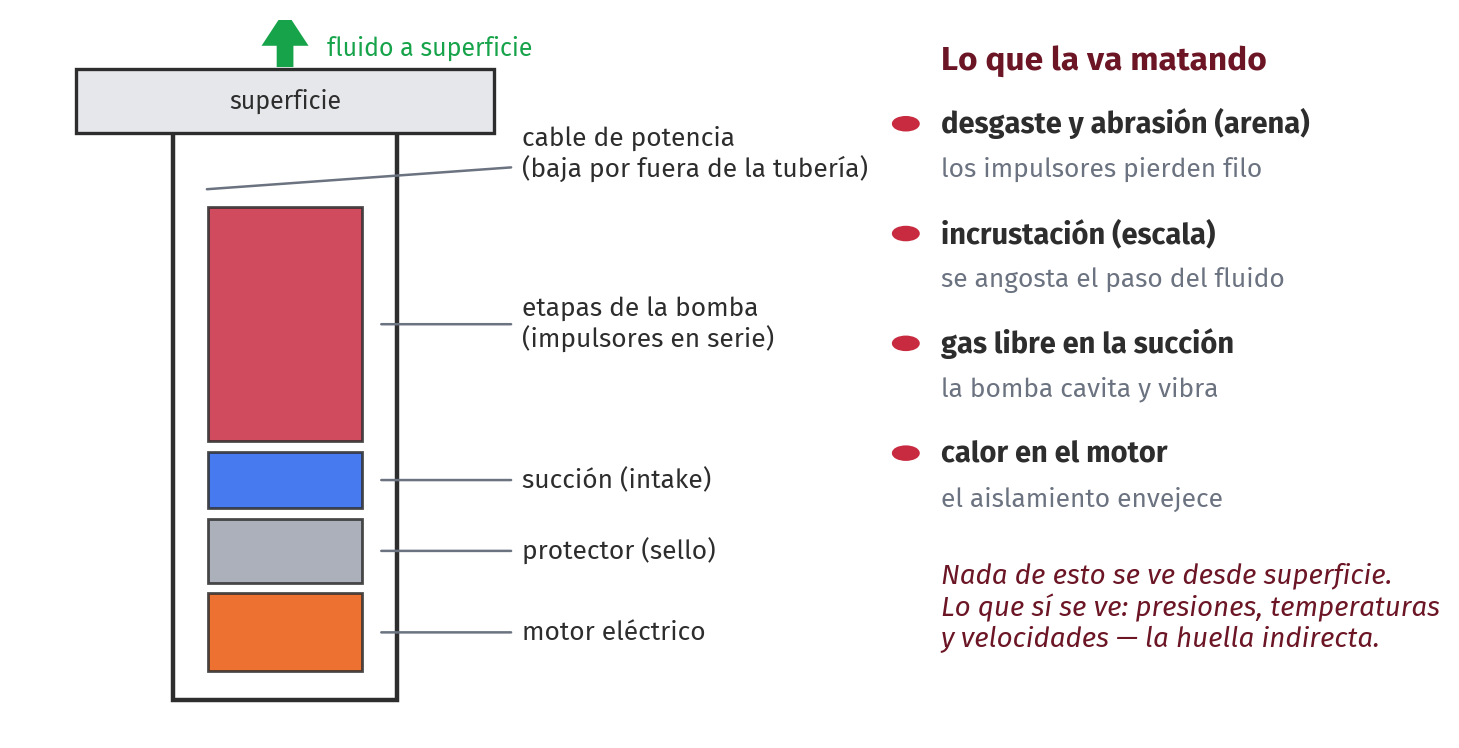
\includegraphics[height=0.62\textheight]{fig_esp.png}
  \end{center}
  \vspace{-2pt}
  {\footnotesize\color{textMuted}
   Una \textbf{ESP} (bomba electrosumergible) es una turbomáquina
   centrífuga: decenas de impulsores en serie girando a miles de RPM,
   colgados a 1.500--3.000 metros, dentro del pozo. \textbf{No se puede ir
   a mirar.} Solo mandan señales.}
\end{frame}

\begin{frame}[shrink=8]{El Día que Se Rompe}
  \vspace{2pt}
  \begin{tcolorbox}[colback=arcaGray, colframe=arcaRed, boxrule=0pt,
    leftrule=4pt, arc=3pt, left=10pt, right=10pt, top=8pt, bottom=8pt]
    {\large\color{arcaDark}\bfseries
     Una ESP no se repara: se \textbf{saca el pozo entero de servicio}
     y se cambia.}\\[6pt]
    {\footnotesize\color{textMuted}
     Matar el pozo, sacar tubería, correr la bomba nueva, volver a
     arrancar. Días de equipo de workover y días de producción diferida
     --- si el cambio estaba \textbf{programado}.}
  \end{tcolorbox}
  \vspace{9pt}
  {\footnotesize\color{textMuted}
   Si \textbf{no} estaba programado, todo empeora: el pozo se queda muerto
   \emph{esperando} equipo (semanas, si hay cola), la falla puede dañar
   cable o tubería, y la producción diferida corre todos esos días.}
  \vspace{7pt}

  {\footnotesize\color{arcaDark}\itshape
   La misma bomba, el mismo cambio --- pero el precio depende de
   \textbf{quién eligió la fecha}: ustedes o la bomba.}
\end{frame}

\begin{frame}[shrink=14]{La Cuenta}
  \vspace{2pt}
  \begin{columns}[T]
    \begin{column}{0.47\textwidth}
      \begin{tcolorbox}[colback=arcaGray, colframe=codeBlue, boxrule=0pt,
        leftrule=4pt, arc=3pt, left=9pt, right=9pt, top=7pt, bottom=7pt]
        {\scriptsize\color{codeBlue}\bfseries CAMBIO PROGRAMADO}\\[6pt]
        {\footnotesize\color{textMuted}
         equipo agendado + 4--6 días\\de producción diferida\\[7pt]}
        {\Large\color{codeBlue}\bfseries 0,3 MUSD}
      \end{tcolorbox}
    \end{column}
    \begin{column}{0.47\textwidth}
      \begin{tcolorbox}[colback=arcaGray, colframe=arcaRed, boxrule=0pt,
        leftrule=4pt, arc=3pt, left=9pt, right=9pt, top=7pt, bottom=7pt]
        {\scriptsize\color{arcaRed}\bfseries FALLA EN OPERACIÓN}\\[6pt]
        {\footnotesize\color{textMuted}
         equipo de emergencia + semanas\\de pozo muerto + daños\\[7pt]}
        {\Large\color{arcaRed}\bfseries 1,5 MUSD}
      \end{tcolorbox}
    \end{column}
  \end{columns}
  \vspace{9pt}
  {\footnotesize\color{textMuted}
   \textbf{Son supuestos, no datos} --- cambian con el campo, el país y el
   contrato de equipos: en tierra puede ser 5 veces menos; costa afuera,
   5 veces más. Lo que suele aguantar es la \textbf{proporción}: la falla
   sorpresa cuesta \textbf{del orden de 5 veces} el cambio programado.}
  \vspace{5pt}

  {\footnotesize\color{arcaDark}\bfseries\itshape
   Los pone finanzas, no el ingeniero. Los dejamos a la vista para que se
   puedan discutir y cambiar --- toda la clase de hoy cuelga de esos dos
   números.}
\end{frame}

\begin{frame}[shrink=8]{Las Tres Políticas Posibles}
  \vspace{2pt}
  {\footnotesize\color{textMuted}
  Con una flota de bombas solo hay tres maneras de decidir \textbf{cuándo}
  cambiar cada una:}
  \vspace{8pt}
  {\footnotesize
    \begin{itemize}\setlength{\itemsep}{10pt}
    \item[{\color{arcaDark}\faBomb}]
      \textbf{Correr a la falla.} No hacer nada hasta que reviente. Se usa
      toda la vida de la bomba\ldots{} y \emph{todas} las fallas son
      de 1,5 MUSD.
    \item[{\color{codeOrange}\faCalendar}]
      \textbf{Calendario.} Cambiarla a una edad fija, digamos la vida
      promedio de la flota. Es la política más común del mundo real.
    \item[{\color{arcaRed}\faHeartbeat}]
      \textbf{Por condición.} Escuchar los sensores de \emph{cada} bomba y
      cambiarla cuando \emph{ella} avise. Para eso hay que saber leer el
      aviso --- y eso es lo que un modelo puede aprender.
    \end{itemize}}
  \vspace{8pt}
  {\scriptsize\color{arcaDark}\itshape
   Hoy las tres compiten con dinero de verdad sobre la misma flota. No
   vamos a suponer cuál gana: lo vamos a \textbf{medir}.}
\end{frame}

\begin{frame}[shrink=14]{El Encargo}
  \vspace{2pt}
  \begin{tcolorbox}[colback=arcaGray, colframe=arcaRed, boxrule=0pt,
    leftrule=4pt, arc=3pt, left=10pt, right=10pt, top=8pt, bottom=8pt]
    {\normalsize\color{arcaDark}\bfseries
     Operamos una flota de 100 unidades. El equipo de intervención hay que
     pedirlo con anticipación y las fallas sorpresa cuestan 5 veces más.}\\[8pt]
    {\normalsize\color{arcaRed}\bfseries
     Para cada unidad: ¿cuánta vida le queda? ¿Cuándo pido el equipo?
     ¿Y cuánto ahorra eso frente al calendario?}
  \end{tcolorbox}
  \vspace{8pt}
  {\footnotesize\color{textMuted}
  Tres entregables, en orden:
  \begin{itemize}\setlength{\itemsep}{5pt}
    \item[{\color{arcaRed}\scriptsize 1.}]
      Un número por unidad: la \textbf{vida útil remanente} (RUL), con su
      versión prudente
    \item[{\color{arcaRed}\scriptsize 2.}]
      Una \textbf{regla de decisión}: cuándo pedir el equipo, y la lista
      del mes
    \item[{\color{arcaRed}\scriptsize 3.}]
      El \textbf{porqué} de cada nombre de la lista --- sin porqué, nadie
      la firma
  \end{itemize}}
\end{frame}

\begin{frame}[shrink=8]{Acotar el Problema (Regla de la Casa)}
  \vspace{-2pt}
  {\footnotesize\color{textMuted}
  \begin{itemize}\setlength{\itemsep}{7pt}
    \item[{\color{codeGreen}\faCheck}]
      \textbf{Dato real, flota real:} 100 turbomáquinas gemelas del
      simulador C-MAPSS de NASA, cada una operada \textbf{desde sana hasta
      la falla}, con 21 sensores. Es el dataset de mantenimiento
      predictivo más estudiado del mundo (PHM 2008).
    \item[{\color{arcaRed}\faBan}]
      \textbf{Lo que NO es:} una flota de ESP. No existe dato público de
      fallas de ESP --- se verificaron ocho fuentes; el registro RIFTS del
      consorcio es cerrado. Lo decimos como es.
    \item[{\color{codeGreen}\faCheck}]
      \textbf{Por qué vale la sustitución:} una ESP \emph{es} una
      turbomáquina --- ejes que giran, degradación progresiva, huella en
      presiones y temperaturas. El \textbf{método} es idéntico; los
      \textbf{costos} que le colgamos sí son de ESP.
    \item[{\color{arcaRed}\faBan}]
      Hoy \textbf{no} dimensionamos bombas ni optimizamos gas lift: la
      decisión de hoy es \emph{cuándo intervenir}. Lo demás se declara al
      cierre.
  \end{itemize}}
  \vspace{5pt}
  {\scriptsize\color{arcaDark}\itshape
   Igual que la C2 dijo «un choke, no una bomba»: la sustitución se
   declara, no se disimula.}
\end{frame}

% ═════════════════════════════════════════════════════════════════════════════
\sectionframe{La Flota y el Reloj}{Cien máquinas corridas hasta la falla, y el número que las ordena \\[6pt] \normalsize 12 -- 40 min}
% ═════════════════════════════════════════════════════════════════════════════

\begin{frame}[shrink=8]{Por Qué Se Degrada una Turbomáquina}
  \vspace{2pt}
  {\footnotesize\color{textMuted}
  La física de la degradación es la misma en una ESP a 2.000 metros y en
  una turbina de NASA:}
  \vspace{7pt}
  {\footnotesize
    \begin{itemize}\setlength{\itemsep}{8pt}
    \item[{\color{arcaRed}\faCog}]
      Las piezas que giran \textbf{se desgastan}: erosión, abrasión,
      holguras que crecen. La máquina pierde \textbf{eficiencia}
      ciclo a ciclo.
    \item[{\color{arcaRed}\faFire}]
      Para entregar el \emph{mismo} trabajo con menos eficiencia, hay que
      \textbf{exigirla más}: sube la temperatura interna, cambia el
      consumo, se mueven las presiones.
    \item[{\color{arcaRed}\faSearch}]
      Nada de eso se ve a simple vista --- pero \textbf{queda escrito en
      los sensores}. La degradación mecánica deja una \emph{huella
      termodinámica}.
    \end{itemize}}
  \vspace{8pt}
  \begin{tcolorbox}[colback=arcaGray, colframe=arcaDark, boxrule=0pt, leftrule=3pt,
    arc=3pt, left=8pt, right=8pt, top=5pt, bottom=5pt]
    {\footnotesize\color{arcaDark}
     La apuesta de la clase entera cabe en una frase: \textbf{si la huella
     está en los sensores, un modelo puede aprender a leerla --- y a decir
     cuánto falta}.}
  \end{tcolorbox}
\end{frame}

\begin{frame}[fragile, shrink=22]{El Archivo}
  \vspace{-4pt}
  \begin{columns}[T]
    \begin{column}{0.56\textwidth}
      \begin{pyblock}
import pandas as pd

url = ("https://raw.githubusercontent"
  ".com/cmosquerat/slb-diplomado/"
  "main/datos/"
  "flota_turbomaquinas_nasa.csv")
d = pd.read_csv(url)

print(d.unidad.nunique(), "unidades")
print(len(d), "filas")
print(d.columns.size, "columnas")
      \end{pyblock}
    \end{column}
    \begin{column}{0.42\textwidth}
      \vspace{2pt}
      \begin{outputblock}
100 unidades
20631 filas
26 columnas
      \end{outputblock}
      \vspace{6pt}
      {\footnotesize\color{textMuted}
      \begin{itemize}\setlength{\itemsep}{5pt}
        \item[{\color{arcaRed}\scriptsize\faArrowRight}]
          Cada fila es \textbf{un ciclo de operación de una unidad}:
          arranque, trabajo, parada
        \item[{\color{arcaRed}\scriptsize\faArrowRight}]
          La unidad 1 tiene 192 filas: vivió 192 ciclos y su última fila
          es \textbf{el día que murió}
        \item[{\color{arcaRed}\scriptsize\faArrowRight}]
          En una ESP el «ciclo» sería un día de operación: misma
          estructura, otro reloj
      \end{itemize}}
    \end{column}
  \end{columns}
\end{frame}

\begin{frame}[shrink=18]{Las Variables, Una a Una}
  \vspace{-2pt}
  {\footnotesize\color{textMuted}
  Tres columnas de identidad y régimen, y 21 sensores con su tag
  industrial. Los que van a importar hoy:}
  \vspace{4pt}
  {\scriptsize
  \begin{center}
  \begin{tabular}{lll}
    \toprule
    \textbf{tag} & \textbf{qué mide} & \textbf{en una ESP sería\ldots} \\
    \midrule
    \texttt{T24}, \texttt{T30} & temperatura en los compresores & temperatura de motor y etapas \\
    \texttt{T50} & temperatura a la salida de la turbina & temperatura de descarga \\
    \texttt{P30}, \texttt{Ps30} & presión tras el compresor & presión de descarga \\
    \texttt{Nf}, \texttt{Nc} & velocidad de los dos ejes & RPM del motor \\
    \texttt{phi} & combustible por unidad de presión & consumo eléctrico por barril \\
    \texttt{BPR} & cuánto flujo se desvía del núcleo & reparto de flujo \\
    \texttt{W31}, \texttt{W32} & flujo de refrigeración & enfriamiento del motor \\
    \bottomrule
  \end{tabular}
  \end{center}}
  \vspace{4pt}
  {\footnotesize\color{textMuted}
   Y las tres de identidad: \texttt{unidad} (cuál máquina), \texttt{ciclo}
   (su edad), \texttt{op\_1..3} (el régimen de operación --- en este
   subconjunto, constante).}
  \vspace{4pt}

  {\scriptsize\color{arcaDark}\itshape
   No hace falta ser experto en turbinas: hace falta saber que cada
   columna es un termómetro o un tacómetro apuntándole a la misma máquina.}
\end{frame}

\begin{frame}[shrink=20]{Antes de Modelar Nada: Mirar el Dato}
  \vspace{-6pt}
  \begin{center}
    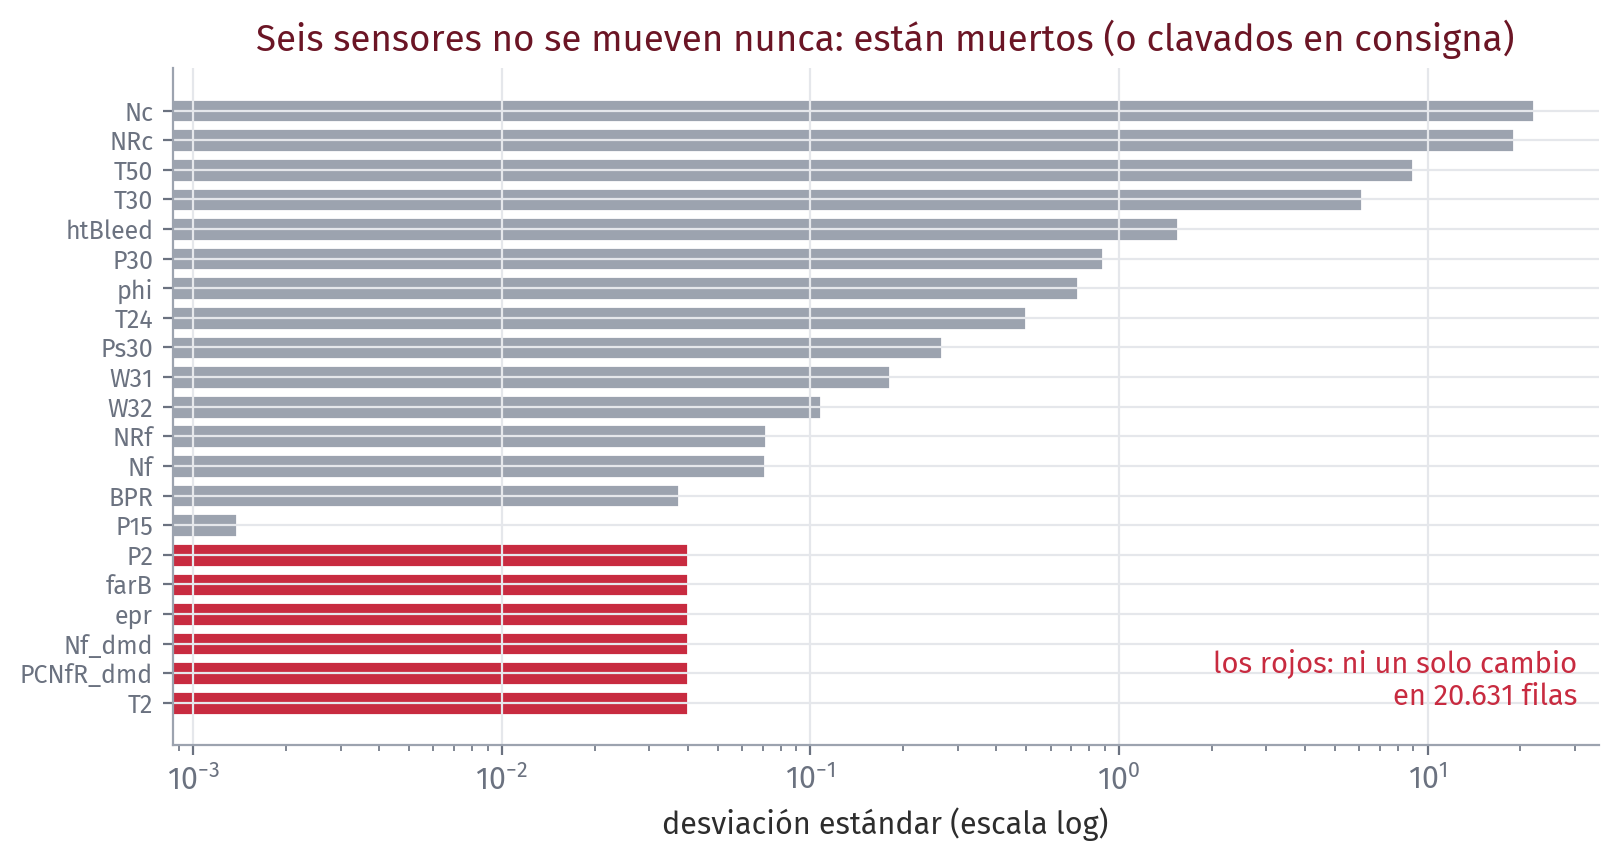
\includegraphics[height=0.60\textheight]{fig_sensores_muertos.png}
  \end{center}
  \vspace{-2pt}
  {\footnotesize\color{textMuted}
   Primer hallazgo del EDA, y nadie lo advierte en la documentación:
   \textbf{6 de los 21 sensores no cambian ni una vez} en 20.631 filas
   (\texttt{T2}, \texttt{P2}, \texttt{epr}, \texttt{farB},
   \texttt{Nf\_dmd}, \texttt{PCNfR\_dmd}). Al modelo no le aportan nada:
   afuera.}
\end{frame}

\begin{frame}[shrink=20]{Cien Vidas, Una Encima de Otra}
  \vspace{-6pt}
  \begin{center}
    
\includegraphics[height=0.60\textheight]{fig_espagueti.png}
  \end{center}
  \vspace{-2pt}
  {\footnotesize\color{textMuted}
   El sensor \texttt{T50} de las 100 unidades. Todas arrancan parecido,
   todas \textbf{suben} hacia el final --- la huella termodinámica ---
   pero cada una a su ritmo, y cada una muere a otra edad.}
\end{frame}

\begin{frame}[shrink=20]{Y Aquí Muere el Calendario Ingenuo}
  \vspace{-6pt}
  \begin{center}
    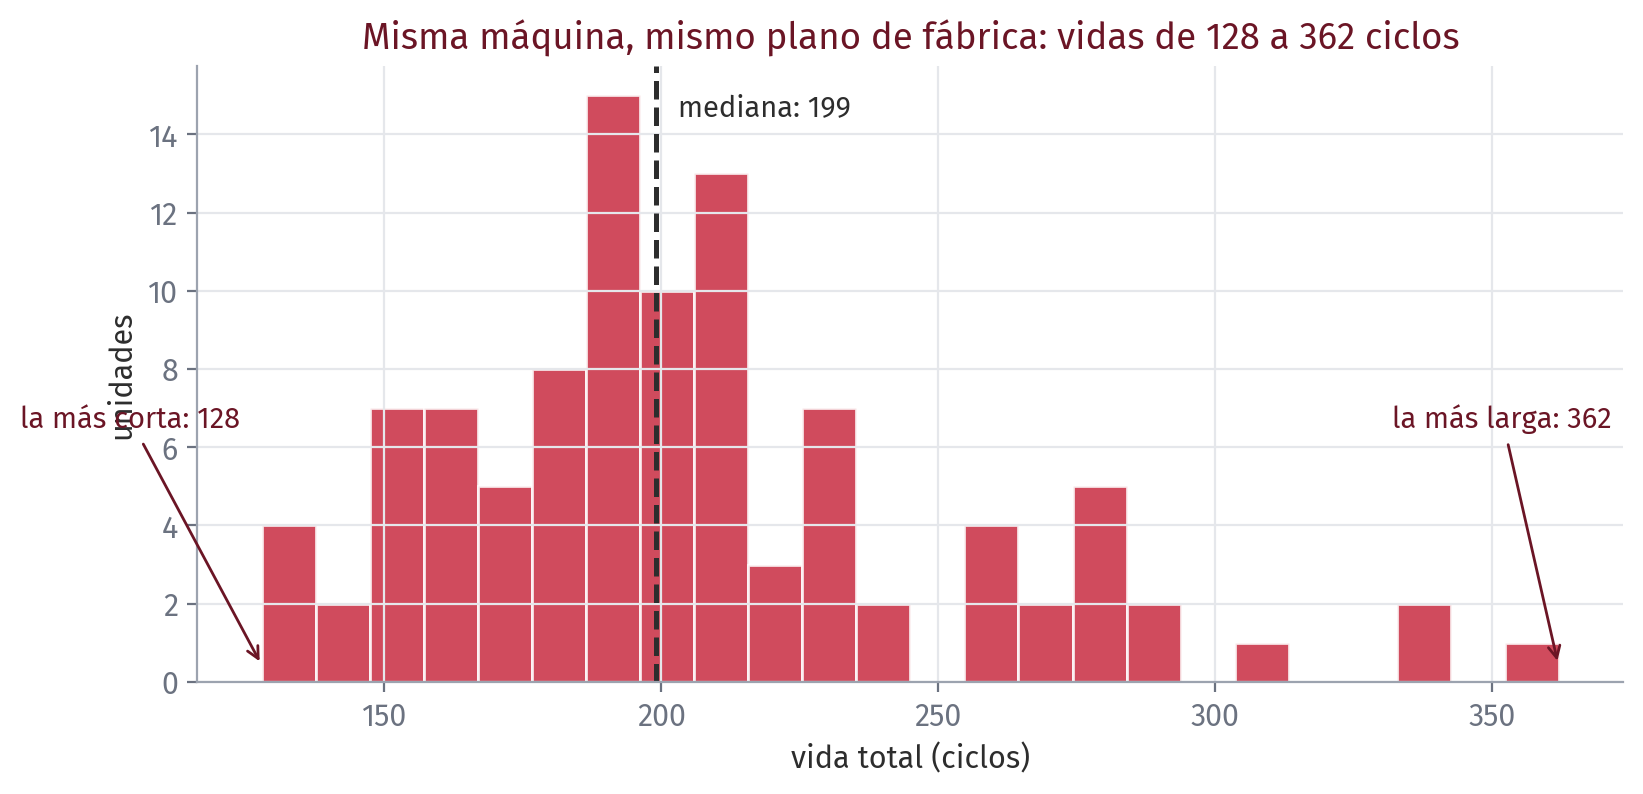
\includegraphics[height=0.58\textheight]{fig_vidas.png}
  \end{center}
  \vspace{-2pt}
  {\footnotesize\color{textMuted}
   Misma máquina, mismo plano de fábrica: la más corta vivió
   \textbf{128 ciclos} y la más larga \textbf{362} --- casi 3 a 1. Un
   calendario a la mediana (199) llega \textbf{tarde} a la mitad de la
   flota y \textbf{bota vida} en la otra mitad. Esto no es un defecto del
   dato: las run life de ESP reales se dispersan igual.}
\end{frame}

\begin{frame}[shrink=20]{La Huella Común: Alinear por la Muerte}
  \vspace{-6pt}
  \begin{center}
    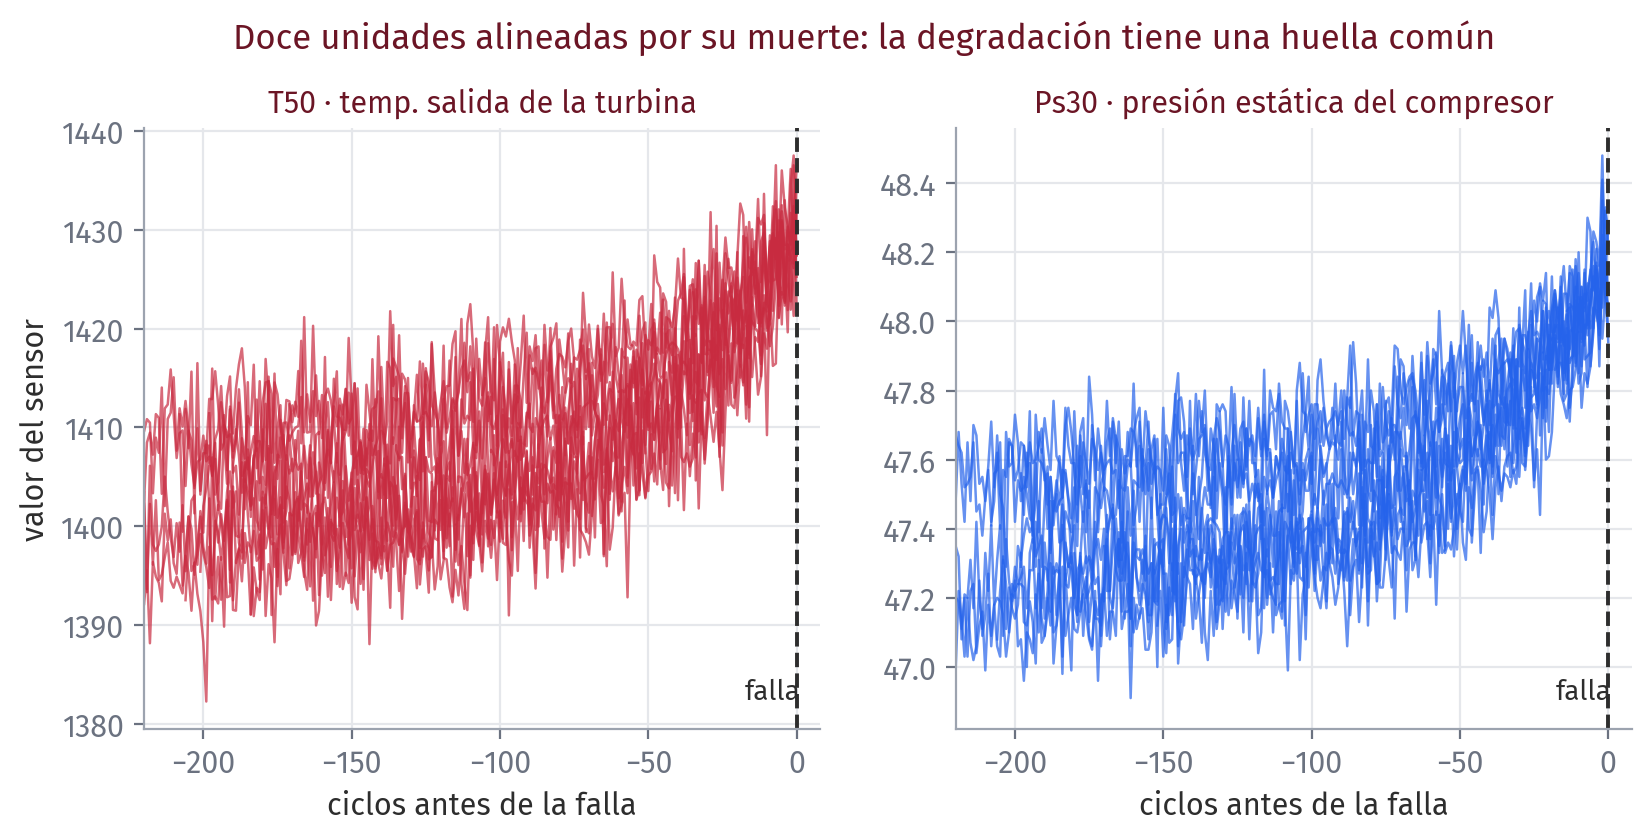
\includegraphics[height=0.58\textheight]{fig_degradacion.png}
  \end{center}
  \vspace{-2pt}
  {\footnotesize\color{textMuted}
   El truco de la C4 (alinear por un evento, no por el calendario), ahora
   alineando por la falla: vistas así, doce unidades cuentan \textbf{la
   misma historia} --- \texttt{T50} sube, \texttt{Ps30} baja. La
   degradación es legible. Queda convertirla en un número.}
\end{frame}

\begin{frame}[shrink=20]{El Número: la Vida Útil Remanente (RUL)}
  \vspace{-6pt}
  \begin{center}
    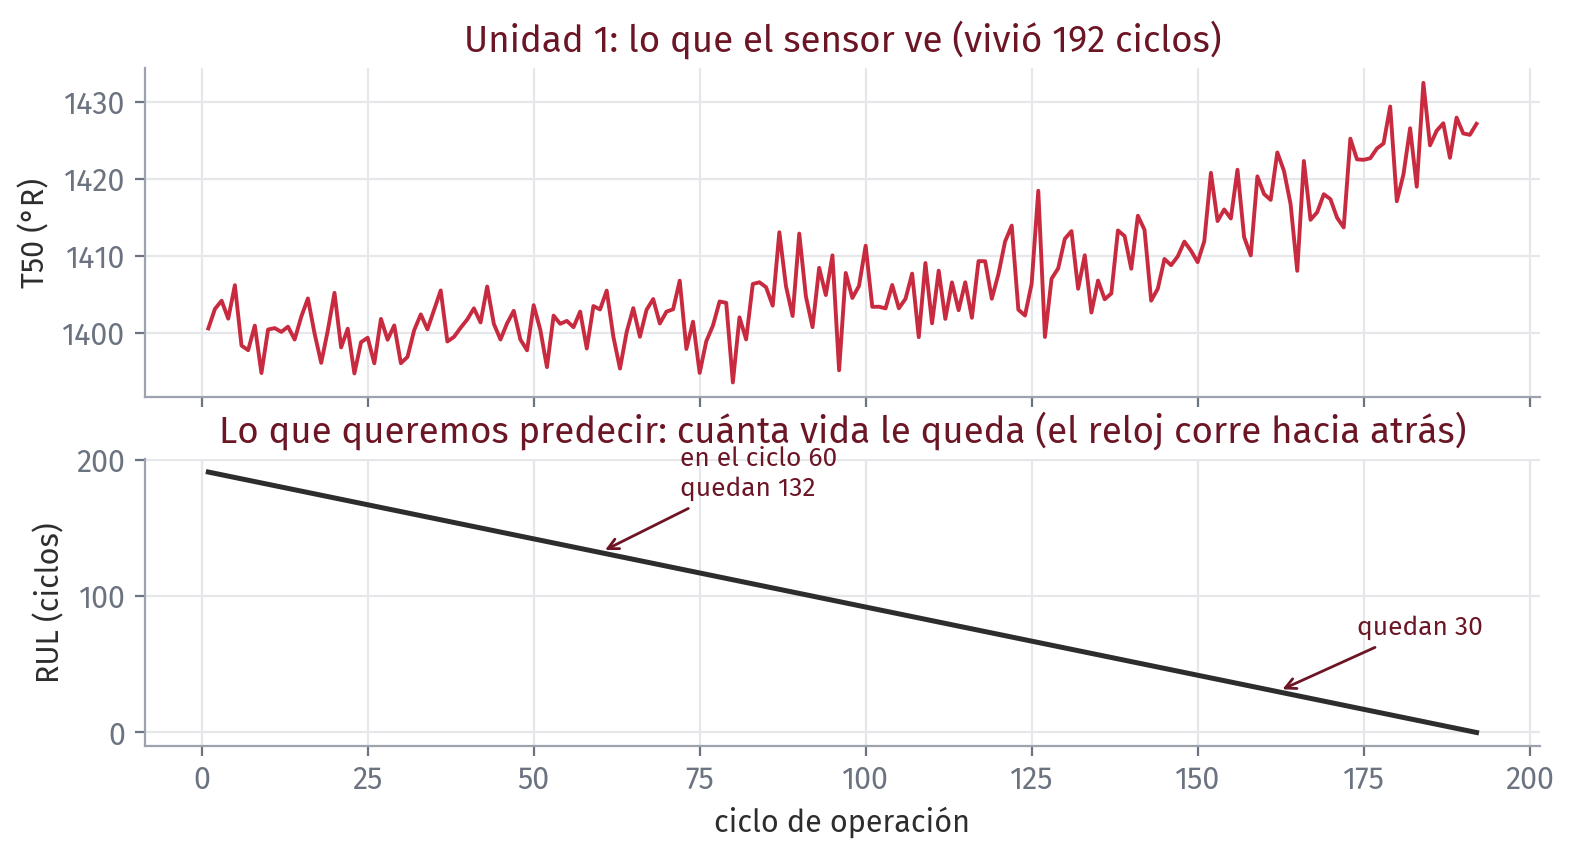
\includegraphics[height=0.58\textheight]{fig_reloj.png}
  \end{center}
  \vspace{-2pt}
  {\footnotesize\color{textMuted}
   \textbf{RUL} (\emph{remaining useful life}): en cada instante, cuántos
   ciclos le faltan a la unidad para morir. Es un reloj que corre hacia
   atrás --- y como estas 100 unidades ya murieron, \textbf{conocemos la
   respuesta correcta en cada fila}: material perfecto para entrenar y
   examinar.}
\end{frame}

\begin{frame}[shrink=18]{RUL, Dicho con Todas Sus Letras}
  \vspace{-2pt}
  {\footnotesize\color{textMuted}
  Vale la pena detenerse, porque este vocabulario es el del mantenimiento
  predictivo en cualquier industria:}
  \vspace{5pt}
  {\scriptsize
  \begin{center}
  \begin{tabular}{p{0.22\textwidth}p{0.68\textwidth}}
    \toprule
    \textbf{término} & \textbf{qué significa, sin adorno} \\
    \midrule
    \textbf{Run life} & La vida total del equipo: de la instalación a la falla. En ESP se mide en días; aquí, en ciclos. Es el número que ya manejan. \\[3pt]
    \textbf{RUL} & \emph{Remaining Useful Life}: cuánta run life \textbf{falta} desde hoy. RUL $=$ vida total $-$ edad. Al instalar, RUL $=$ run life; el día de la falla, RUL $=$ 0. \\[3pt]
    \textbf{Falla funcional} & El momento en que el equipo ya no cumple su función (la bomba no levanta caudal), no necesariamente la rotura total. Ahí termina el reloj. \\[3pt]
    \textbf{Prognosis (PHM)} & La disciplina que estima RUL desde sensores. Es la evolución del \emph{monitoreo}: detectar dice «está enferma»; prognosis dice «cuánto le queda». \\[3pt]
    \textbf{Mant. por condición} & La política que decide con el estado medido de \emph{cada} equipo --- lo opuesto al calendario. Necesita la prognosis para planear. \\
    \bottomrule
  \end{tabular}
  \end{center}}
  \vspace{4pt}
  {\scriptsize\color{arcaDark}\itshape
   La física que hace todo esto posible: la degradación mecánica es
   \textbf{gradual y acumulativa} --- desgaste, erosión, fatiga avanzan
   ciclo a ciclo, no de golpe --- y cada avance \textbf{mueve variables
   termodinámicas medibles}. Por eso el RUL se puede estimar. Cuando la
   falla es súbita y sin precursor (un rayo, un golpe), no hay RUL que
   valga: ningún modelo ve lo que no deja huella.}
\end{frame}

\begin{frame}[fragile, shrink=22]{El Reloj, en Código}
  \vspace{-4pt}
  \begin{columns}[T]
    \begin{column}{0.56\textwidth}
      \begin{pyblock}
vida = (d.groupby("unidad")
         .ciclo.max())

d = d.join(vida.rename("vida"),
           on="unidad")
d["rul"] = d.vida - d.ciclo

d.loc[d.unidad == 1,
      ["ciclo", "vida", "rul"]
     ].iloc[[0, 100, -1]]
      \end{pyblock}
    \end{column}
    \begin{column}{0.42\textwidth}
      \vspace{2pt}
      \begin{outputblock}
     ciclo  vida  rul
0        1   192  191
100    101   192   91
191    192   192    0
      \end{outputblock}
      \vspace{6pt}
      {\footnotesize\color{textMuted}
      \begin{itemize}\setlength{\itemsep}{5pt}
        \item[{\color{arcaRed}\scriptsize\faArrowRight}]
          \texttt{groupby().max()} $\rightarrow$ la vida de cada unidad:
          su último ciclo
        \item[{\color{arcaRed}\scriptsize\faArrowRight}]
          \texttt{vida - ciclo} $\rightarrow$ el reloj: empieza en la vida
          y termina en \textbf{0} el día de la falla
        \item[{\color{arcaRed}\scriptsize\faArrowRight}]
          Tres líneas --- y el problema ya es de \textbf{regresión}, como
          los del M3·C1
      \end{itemize}}
    \end{column}
  \end{columns}
\end{frame}

\begin{frame}[shrink=16]{De Señales a Tabla, Otra Vez}
  \vspace{-2pt}
  {\footnotesize\color{textMuted}
  Regla de la C2, que hoy se recicla entera: \textbf{los modelos no comen
  señales, comen tablas}. Para cada fila, tres miradas por sensor:}
  \vspace{7pt}
  {\footnotesize
    \begin{itemize}\setlength{\itemsep}{8pt}
    \item[{\color{arcaRed}\faCamera}]
      \textbf{El valor de hoy} (\texttt{T50}): la foto instantánea ---
      con su ruido encima
    \item[{\color{arcaRed}\faFilter}]
      \textbf{La media de los últimos 20 ciclos} (\texttt{T50\_m}): la
      misma foto, sin temblor --- la media móvil del M2, al trabajo
    \item[{\color{arcaRed}\faChartLine}]
      \textbf{La pendiente de esa media} (\texttt{T50\_d}): ¿está
      subiendo o bajando? --- la \emph{dirección} del deterioro
    \end{itemize}}
  \vspace{7pt}
  \begin{tcolorbox}[colback=arcaGray, colframe=arcaDark, boxrule=0pt, leftrule=3pt,
    arc=3pt, left=8pt, right=8pt, top=5pt, bottom=5pt]
    {\footnotesize\color{arcaDark}
     15 sensores vivos $\times$ 3 miradas $+$ la edad de la unidad
     $=$ \textbf{46 columnas}. Muchas unidades, muchas variables: el
     terreno donde el módulo ya midió que el ML cobra.}
  \end{tcolorbox}
  \vspace{5pt}
  {\scriptsize\color{arcaDark}\itshape
   ¿Por qué darle la edad? Porque el calendario la usa --- y el modelo
   tiene que poder ganarle \textbf{con sus mismas armas y mejores ojos}.
   Al final vamos a auditar cuánto la usó de verdad.}
\end{frame}

\begin{frame}[shrink=8]{La Trampa de Siempre, por Última Vez}
  \vspace{2pt}
  {\footnotesize\color{textMuted}
  Vamos a apartar \textbf{25 unidades completas} antes de tocar nada.
  Entrenamos con 75, y las 25 apartadas solo se destapan al final.}
  \vspace{8pt}
  \begin{columns}[T]
    \begin{column}{0.48\textwidth}
      \begin{tcolorbox}[colback=arcaGray, colframe=arcaRed, boxrule=0pt, leftrule=3pt,
        arc=3pt, left=8pt, right=8pt, top=5pt, bottom=5pt]
        {\scriptsize\color{arcaRed}\bfseries\faBan\hspace{4pt}PARTIR POR FILAS}\\[5pt]
        {\scriptsize\color{textMuted}
         Filas de la \emph{misma} unidad caen en entrenamiento \textbf{y}
         en examen. El modelo «reconoce» a la unidad --- el ciclo 130 de
         la unidad 5 delata a su ciclo 131 --- y el examen sale
         mentirosamente bien.}
      \end{tcolorbox}
    \end{column}
    \begin{column}{0.48\textwidth}
      \begin{tcolorbox}[colback=arcaGray, colframe=codeGreen, boxrule=0pt, leftrule=3pt,
        arc=3pt, left=8pt, right=8pt, top=5pt, bottom=5pt]
        {\scriptsize\color{codeGreen}\bfseries\faCheck\hspace{4pt}PARTIR POR UNIDAD}\\[5pt]
        {\scriptsize\color{textMuted}
         La unidad entra \textbf{entera} a un solo lado. El examen imita
         la vida real: pronosticar una máquina que \textbf{jamás se ha
         visto}. Es el \texttt{GroupKFold} de la C2 y el «sacar el campo
         entero» de la C3.}
      \end{tcolorbox}
    \end{column}
  \end{columns}
  \vspace{8pt}
  {\scriptsize\color{arcaDark}\itshape
   Tercera clase seguida con la misma trampa. No es casualidad: es
   \textbf{el} error que más informes de ML entierra en esta industria.}
\end{frame}
% ═════════════════════════════════════════════════════════════════════════════
\sectionframe{El Modelo que Faltaba}{El calendario como rival, y la cadena que corrige sus propios errores \\[6pt] \normalsize 40 -- 70 min}
% ═════════════════════════════════════════════════════════════════════════════

\begin{frame}[shrink=6]{El Rival No Es un Muñeco de Paja: Es la Política Real}
  \vspace{-6pt}
  \begin{center}
    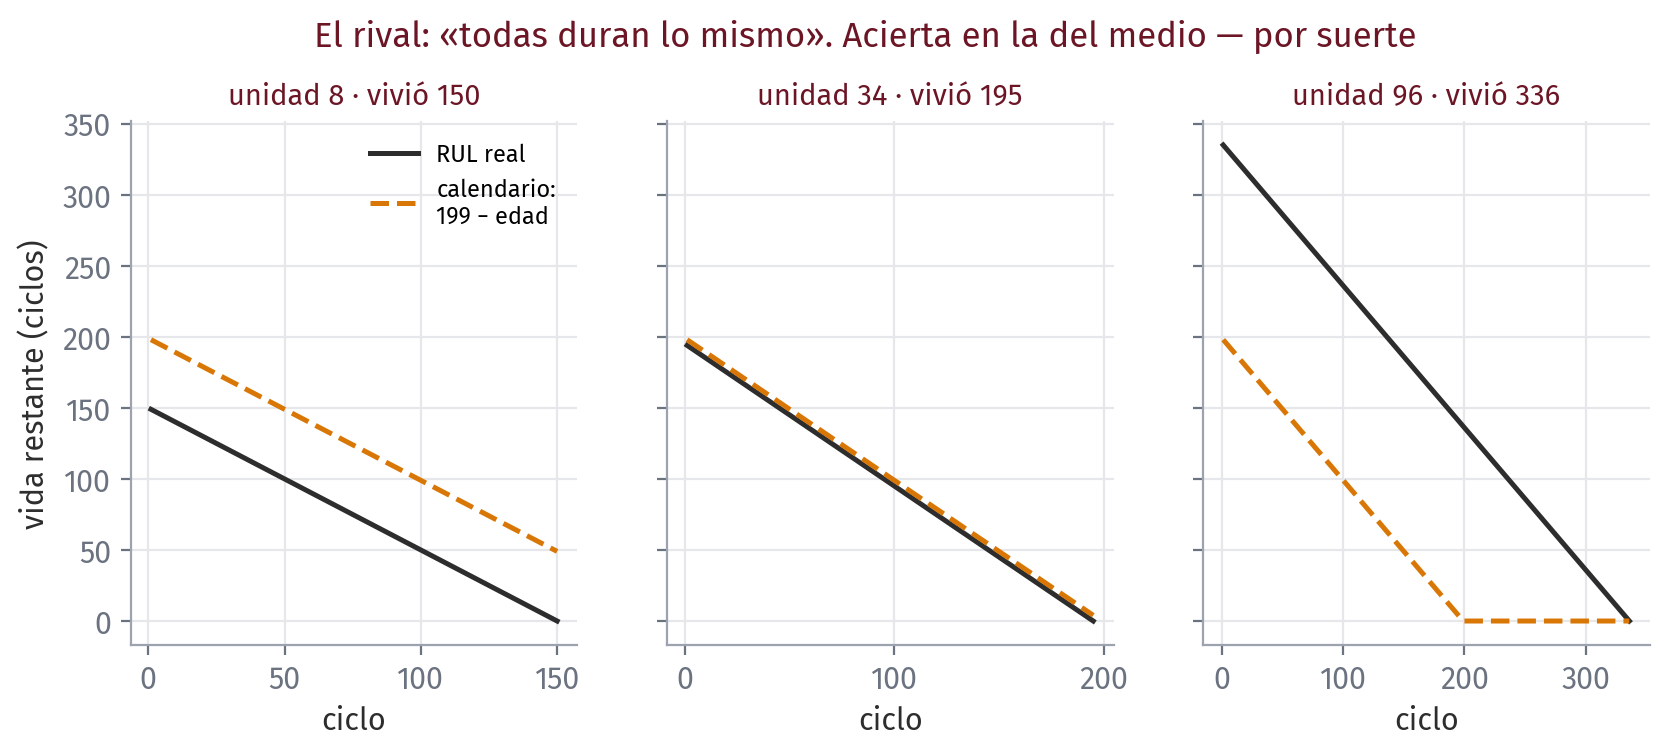
\includegraphics[height=0.52\textheight]{fig_rival.png}
  \end{center}
  \vspace{-2pt}
  {\footnotesize\color{textMuted}
   El modelo tonto de hoy: \textbf{RUL $=$ 199 $-$ edad} (la mediana de la
   flota menos los ciclos corridos). Eso no es un invento académico:
   \textbf{es literalmente el mantenimiento por calendario} que corre en
   media industria. Ganarle al tonto $=$ justificar el proyecto frente a
   la política vigente.}
\end{frame}

\begin{frame}[shrink=8]{El Récord a Batir}
  \vspace{-4pt}
  {\small\color{arcaDark}\bfseries
   Corrimos el calendario sobre las 25 unidades apartadas. Esto es lo que
   hay que superar:}
  \vspace{10pt}
  \begin{columns}[T]
    \begin{column}{0.31\textwidth}
      \begin{tcolorbox}[colback=arcaGray, colframe=arcaDark, boxrule=0pt, leftrule=3pt,
        arc=3pt, left=6pt, right=6pt, top=6pt, bottom=6pt]
        \centering
        {\scriptsize\color{textMuted}ERROR, TODA LA VIDA}\\[4pt]
        {\LARGE\color{arcaDark}\bfseries 35 ciclos}\\[4pt]
        {\scriptsize\color{textMuted}de equivocación media\\al estimar el RUL}
      \end{tcolorbox}
    \end{column}
    \begin{column}{0.31\textwidth}
      \begin{tcolorbox}[colback=arcaGray, colframe=arcaRed, boxrule=0pt, leftrule=3pt,
        arc=3pt, left=6pt, right=6pt, top=6pt, bottom=6pt]
        \centering
        {\scriptsize\color{textMuted}CUANDO QUEDAN $<$ 50}\\[4pt]
        {\LARGE\color{arcaRed}\bfseries 21 ciclos}\\[4pt]
        {\scriptsize\color{textMuted}de error justo cuando\\hay que decidir}
      \end{tcolorbox}
    \end{column}
    \begin{column}{0.31\textwidth}
      \begin{tcolorbox}[colback=arcaGray, colframe=codeBlue, boxrule=0pt, leftrule=3pt,
        arc=3pt, left=6pt, right=6pt, top=6pt, bottom=6pt]
        \centering
        {\scriptsize\color{textMuted}SI SE LE HACE CASO}\\[4pt]
        {\LARGE\color{codeBlue}\bfseries 14 de 25}\\[4pt]
        {\scriptsize\color{textMuted}unidades revientan antes\\de su cita de cambio}
      \end{tcolorbox}
    \end{column}
  \end{columns}
  \vspace{10pt}
  {\footnotesize\color{arcaDark}\itshape
   Fíjense en la tercera caja: un error de RUL no es un número
   abstracto. \textbf{Equivocarse por arriba significa una bomba muerta
   esperando equipo.} Volveremos a eso con dólares.}
\end{frame}

\begin{frame}[shrink=16]{Qué Falta en la Caja de Herramientas}
  \vspace{2pt}
  {\footnotesize\color{textMuted}
  El diplomado ya les dio: regresión lineal y logística (M3), árboles y
  \textbf{Random Forest} (M3), SVM (M3), K-means (M4). ¿Qué agujero
  queda?}
  \vspace{8pt}
  \begin{tcolorbox}[colback=arcaGray, colframe=arcaRed, boxrule=0pt,
    leftrule=4pt, arc=3pt, left=10pt, right=10pt, top=7pt, bottom=7pt]
    {\footnotesize\color{arcaDark}
     El Random Forest es un \textbf{comité}: mil árboles opinan
     \textbf{en paralelo}, cada uno por su lado, y se promedia.\\[6pt]
     Nadie del comité ve los errores de los demás. ¿Y si en vez de
     promediar opiniones independientes, cada árbol nuevo
     \textbf{corrigiera lo que el anterior dejó mal}?}
  \end{tcolorbox}
  \vspace{8pt}
  {\footnotesize\color{textMuted}
   Esa idea --- árboles \textbf{en serie}, cada uno entrenado sobre el
   error del acumulado --- se llama \textbf{gradient boosting}. Es el
   modelo que desde hace una década gana casi todo lo que se juega con
   \textbf{datos tabulares} (filas $\times$ columnas), y el que más corre
   en producción en la industria.}
  \vspace{6pt}

  {\scriptsize\color{arcaDark}\itshape
   Hoy lo abrimos despacio, como hicimos con el bosque en el M3: primero
   la idea con dibujos, después el código, después el examen.}
\end{frame}

\begin{frame}[shrink=26]{Un Paso de la Cadena, en Cámara Lenta}
  \vspace{-6pt}
  \begin{center}
    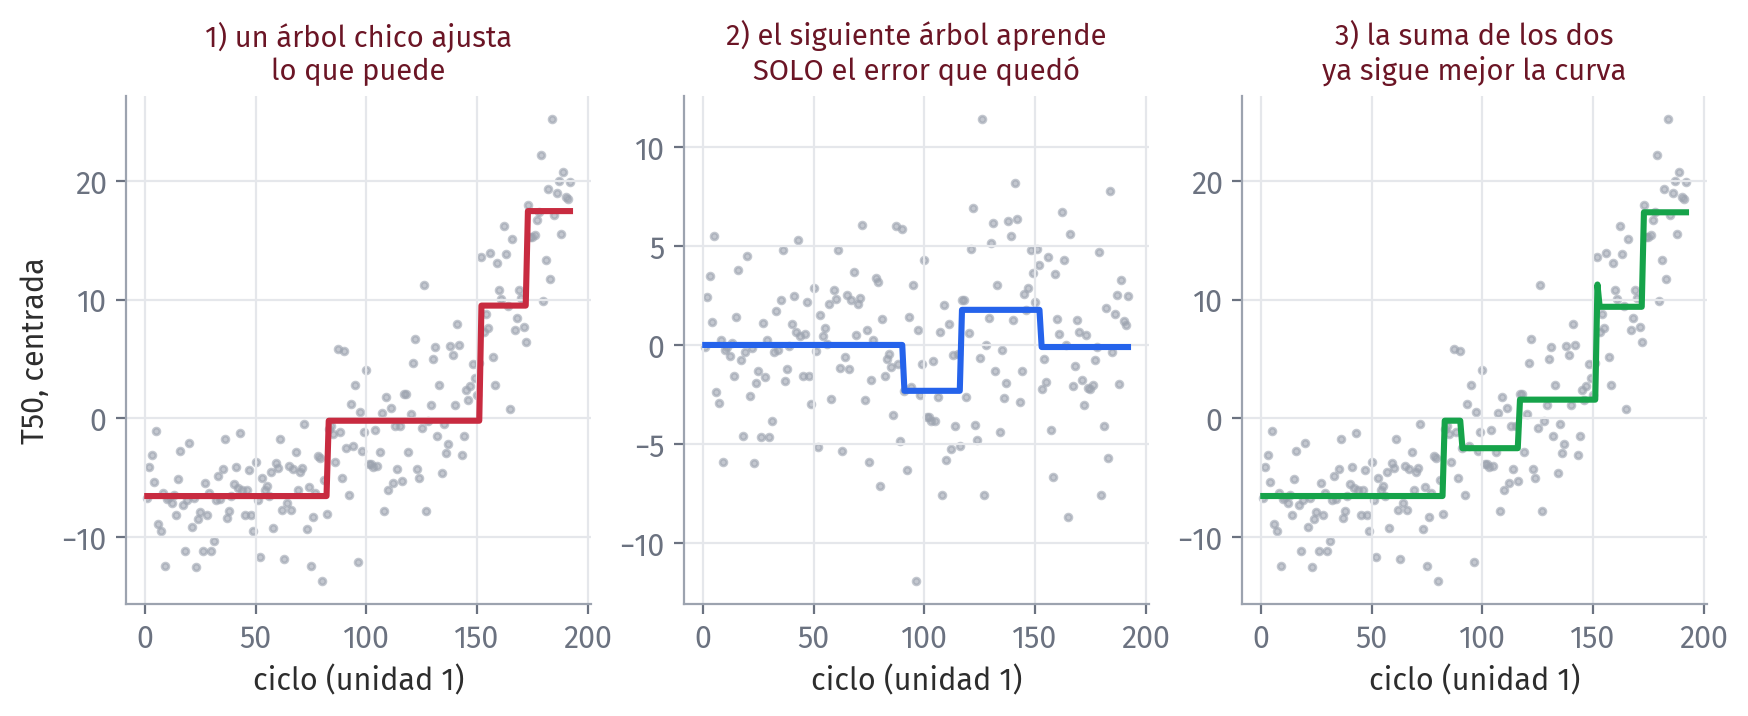
\includegraphics[height=0.46\textheight]{fig_boost_paso.png}
  \end{center}
  \vspace{0pt}
  {\footnotesize\color{textMuted}
   El segundo árbol \textbf{no ve los datos: ve los errores del primero}.
   Boosting es repetir esa corrección cientos de veces.}
\end{frame}

\begin{frame}[shrink=6]{La Cadena Completa: 1, 10, 300 Árboles}
  \vspace{-6pt}
  \begin{center}
    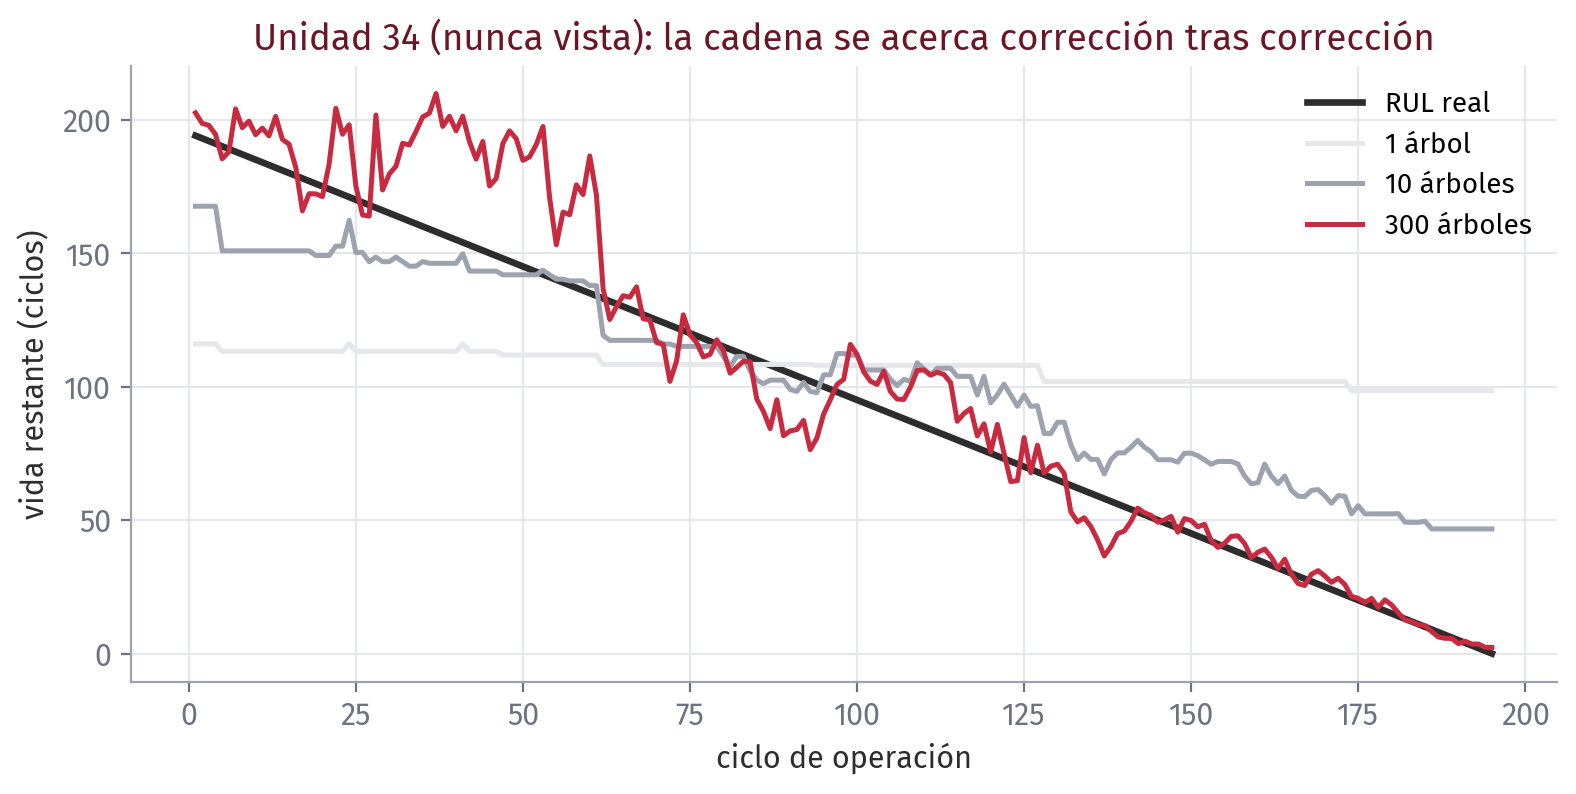
\includegraphics[height=0.56\textheight]{fig_boost_arboles.png}
  \end{center}
  \vspace{-2pt}
  {\footnotesize\color{textMuted}
   El RUL de la unidad 34 (apartada: el modelo jamás la vio). Con 1 árbol,
   una escalera burda; con 10, la forma aparece; con 300, sigue el reloj
   --- incluso el codo donde la degradación se acelera.}
\end{frame}

\begin{frame}[shrink=8]{Por Qué se Llama «Gradiente», Sin Álgebra}
  \vspace{2pt}
  {\footnotesize\color{textMuted}
  \begin{itemize}\setlength{\itemsep}{8pt}
    \item[{\color{arcaRed}\faMountain}]
      Imaginen el error total del modelo como una \textbf{montaña}: la
      cima es «me equivoco mucho», el valle es «me equivoco poco».
    \item[{\color{arcaRed}\faShoePrints}]
      Cada árbol nuevo es \textbf{un paso cuesta abajo}: apunta en la
      dirección que más reduce el error \emph{en este momento}. «Gradiente»
      es solo el nombre técnico de esa dirección.
    \item[{\color{arcaRed}\faSlidersH}]
      Y hay una perilla: el \textbf{tamaño del paso} (\emph{learning
      rate}). Pasos grandes bajan rápido pero se pasan de largo; pasos
      chicos llegan más lejos --- si la cadena es larga.
  \end{itemize}}
  \vspace{6pt}
  \begin{center}
    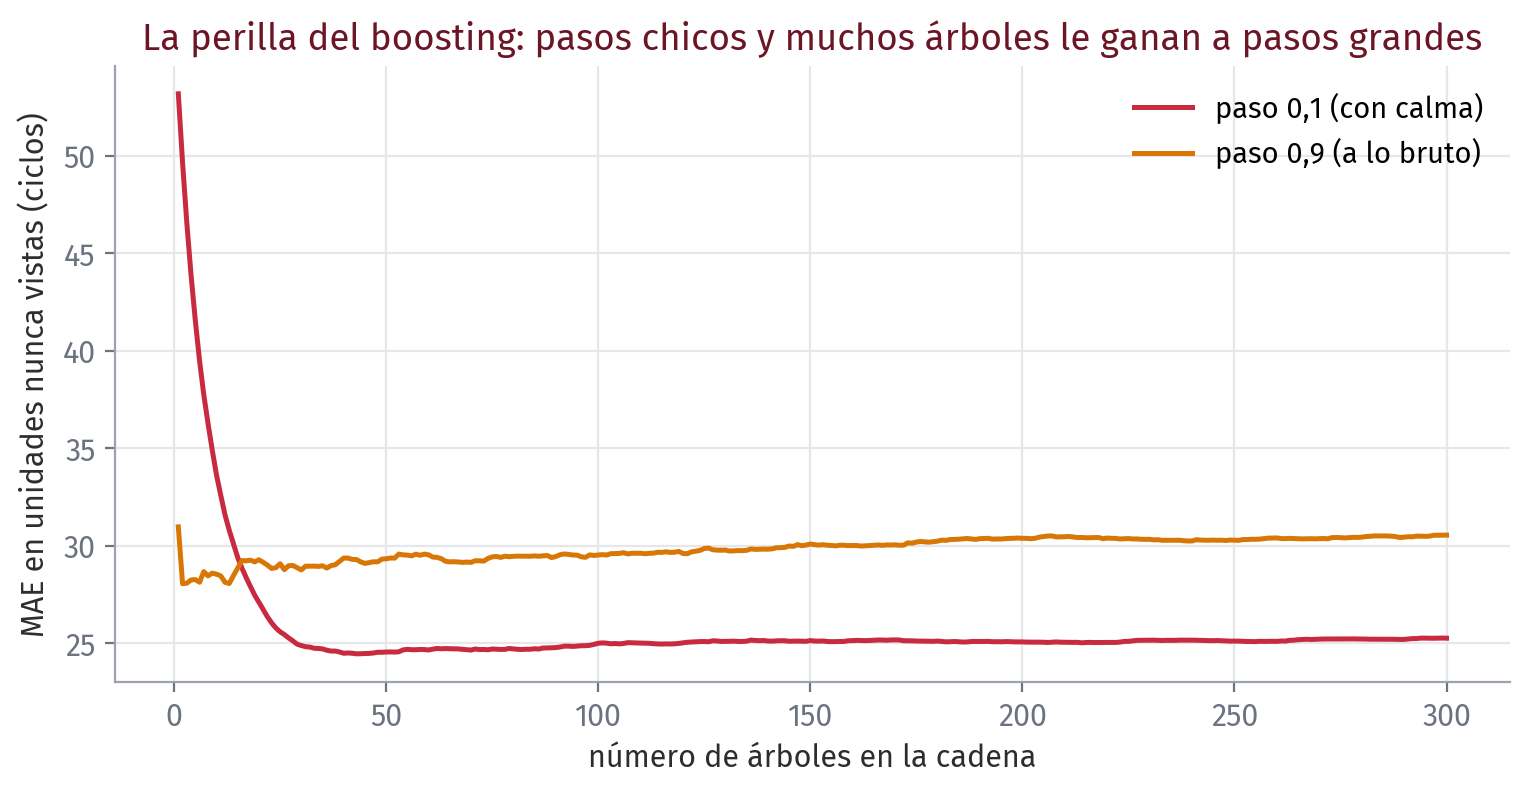
\includegraphics[height=0.40\textheight]{fig_perilla.png}
  \end{center}
\end{frame}

\begin{frame}[shrink=8]{El Estado del Arte, con Fecha y con Límites}
  \vspace{2pt}
  {\footnotesize\color{textMuted}
  Digámoslo con precisión, porque «estado del arte» se dice mucho y se
  mide poco:}
  \vspace{7pt}
  {\footnotesize
    \begin{itemize}\setlength{\itemsep}{8pt}
    \item[{\color{codeGreen}\faCheck}]
      En \textbf{datos tabulares} --- filas y columnas, como los de toda
      esta industria --- el gradient boosting (XGBoost 2016, LightGBM
      2017) domina las competencias y la producción \textbf{desde hace
      una década}, y los estudios comparativos serios lo siguen
      confirmando frente a redes neuronales.
    \item[{\color{arcaRed}\faBan}]
      En \textbf{imagen, texto y señal cruda}, ganan las redes profundas
      --- ahí el boosting no compite.
    \item[{\color{codeGreen}\faCheck}]
      Nuestra tabla de hoy: 20.631 filas $\times$ 46 columnas.
      \textbf{Territorio boosting.}
    \end{itemize}}
  \vspace{7pt}
  \begin{tcolorbox}[colback=arcaGray, colframe=arcaDark, boxrule=0pt, leftrule=3pt,
    arc=3pt, left=8pt, right=8pt, top=5pt, bottom=5pt]
    {\footnotesize\color{arcaDark}\itshape
     Traducción práctica: antes de pensar en una red neuronal para un
     problema de tabla en su campo, el boosting es \textbf{el listón que
     esa red tendría que superar} --- y casi nunca lo supera.}
  \end{tcolorbox}
\end{frame}

\begin{frame}[fragile, shrink=22]{El Modelo, en Código}
  \vspace{-4pt}
  \begin{columns}[T]
    \begin{column}{0.56\textwidth}
      \begin{pyblock}
from sklearn.ensemble import (
  HistGradientBoostingRegressor)

m = HistGradientBoostingRegressor(
      max_iter=300,      # arboles
      learning_rate=0.03,  # paso
      random_state=0)

m.fit(X_tr, y_tr)        # 75 unid.
rul_hat = m.predict(X_te)  # 25 unid.
      \end{pyblock}
    \end{column}
    \begin{column}{0.42\textwidth}
      \vspace{2pt}
      {\footnotesize\color{textMuted}
      \begin{itemize}\setlength{\itemsep}{6pt}
        \item[{\color{arcaRed}\scriptsize\faArrowRight}]
          \texttt{Hist\ldots} es el gradient boosting \textbf{moderno} de
          scikit-learn: la misma idea de la cadena, con histogramas para
          ir rápido (la técnica de LightGBM)
        \item[{\color{arcaRed}\scriptsize\faArrowRight}]
          \texttt{max\_iter} $\rightarrow$ el largo de la cadena;
          \texttt{learning\_rate} $\rightarrow$ el tamaño del paso
        \item[{\color{arcaRed}\scriptsize\faArrowRight}]
          La interfaz es \textbf{idéntica} a todo lo que ya usaron:
          \texttt{fit} / \texttt{predict}. Cambiar de modelo cuesta una
          línea
      \end{itemize}}
    \end{column}
  \end{columns}
\end{frame}

\begin{frame}[shrink=16]{Las Perillas No Se Giran a Ojo}
  \vspace{2pt}
  {\footnotesize\color{textMuted}
  ¿Y de dónde salió \texttt{learning\_rate=0.03}? \textbf{No de la
  intuición}: de un examen. Eso es el \emph{hyperparameter tuning}, y
  tiene tres reglas que valen más que cualquier receta:}
  \vspace{7pt}
  {\footnotesize
    \begin{itemize}\setlength{\itemsep}{8pt}
    \item[{\color{arcaRed}\scriptsize 1.}]
      \textbf{Se prueba una malla, no una corazonada}: todas las
      combinaciones de paso $\{0{,}03,\ 0{,}1,\ 0{,}3\}$ $\times$
      profundidad $\{2,\ 3,\ \text{libre}\}$
    \item[{\color{arcaRed}\scriptsize 2.}]
      Cada celda se califica con \textbf{validación cruzada por unidad}
      (el \texttt{GroupKFold} de hace un rato): 5 exámenes por celda,
      máquinas nunca vistas en cada uno
    \item[{\color{arcaRed}\scriptsize 3.}]
      Todo ocurre \textbf{dentro de las 75 de entrenamiento}. Las 25
      apartadas \emph{no votan}: si la malla las viera, el examen final
      quedaría contaminado
    \end{itemize}}
  \vspace{7pt}
  \begin{tcolorbox}[colback=arcaGray, colframe=arcaDark, boxrule=0pt, leftrule=3pt,
    arc=3pt, left=8pt, right=8pt, top=5pt, bottom=5pt]
    {\footnotesize\color{arcaDark}
     En código son cuatro líneas: \texttt{GridSearchCV(modelo, malla,
     cv=folds\_por\_unidad)}. Lo difícil no es la sintaxis: es
     \textbf{resistir la tentación de elegir con el test}.}
  \end{tcolorbox}
\end{frame}

\begin{frame}[shrink=20]{El Resultado de la Malla --- y una Lección Incómoda}
  \vspace{-6pt}
  \begin{center}
    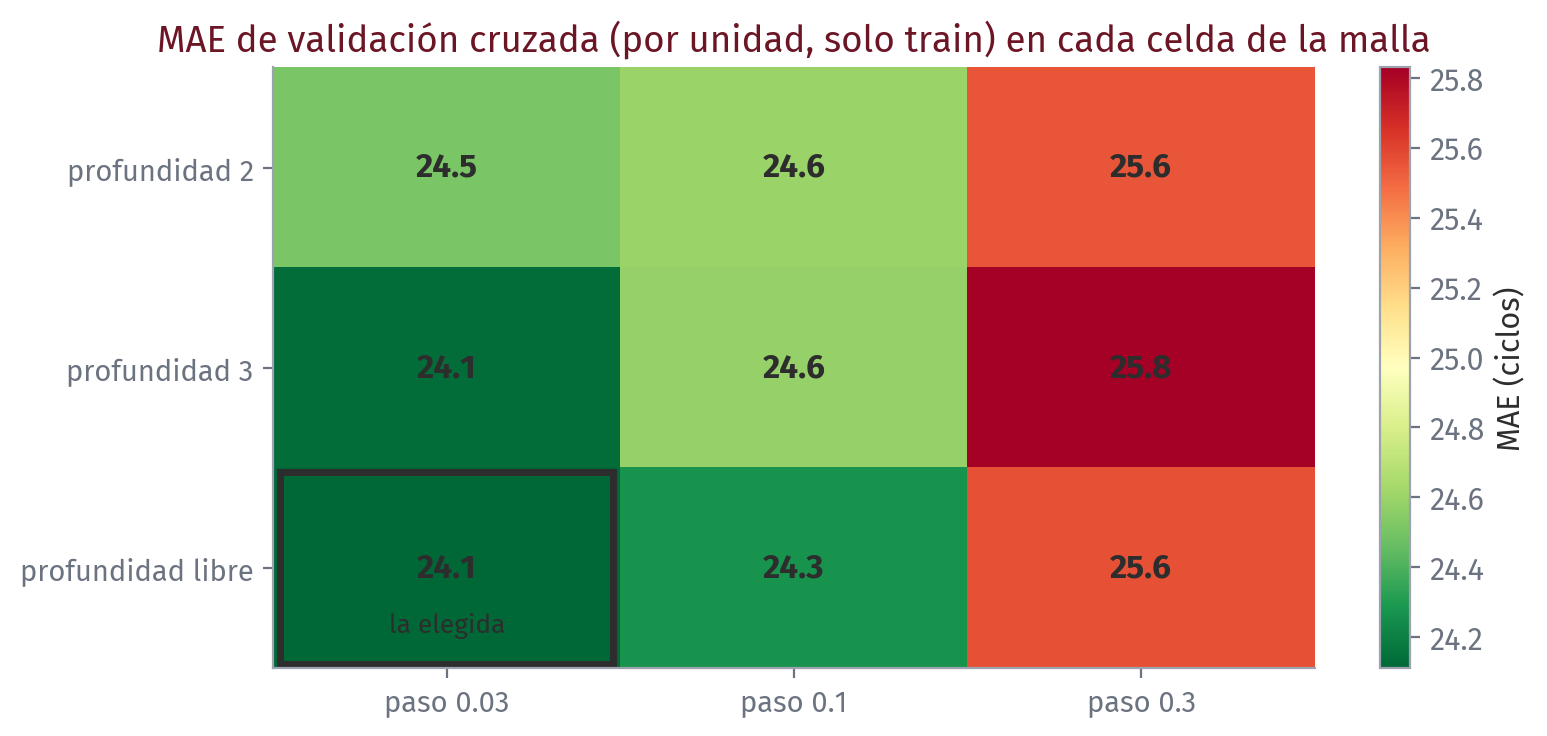
\includegraphics[height=0.54\textheight]{fig_malla.png}
  \end{center}
  \vspace{-2pt}
  {\footnotesize\color{textMuted}
   Toda la malla vive entre \textbf{24,1 y 25,8 ciclos}; la celda elegida
   le gana al default de sklearn por \textbf{0,2}. La lección honesta: el
   afinado fino compra \emph{poco} --- los saltos grandes los dieron
   \textbf{el modelo correcto y los features correctos}. Afinen al final,
   no primero.}
\end{frame}

\begin{frame}[shrink=6]{El Marcador}
  \vspace{-6pt}
  \begin{center}
    
\includegraphics[height=0.56\textheight]{fig_marcador.png}
  \end{center}
  \vspace{-2pt}
  {\footnotesize\color{textMuted}
   En las 25 unidades nunca vistas: el calendario se equivoca por
   \textbf{35 ciclos}, el boosting por \textbf{24}. Gana --- pero el
   marcador global esconde lo importante. Hay que mirar \emph{dónde}
   se gana.}
\end{frame}

\begin{frame}[shrink=20]{La Zona de la Decisión}
  \vspace{-6pt}
  \begin{center}
    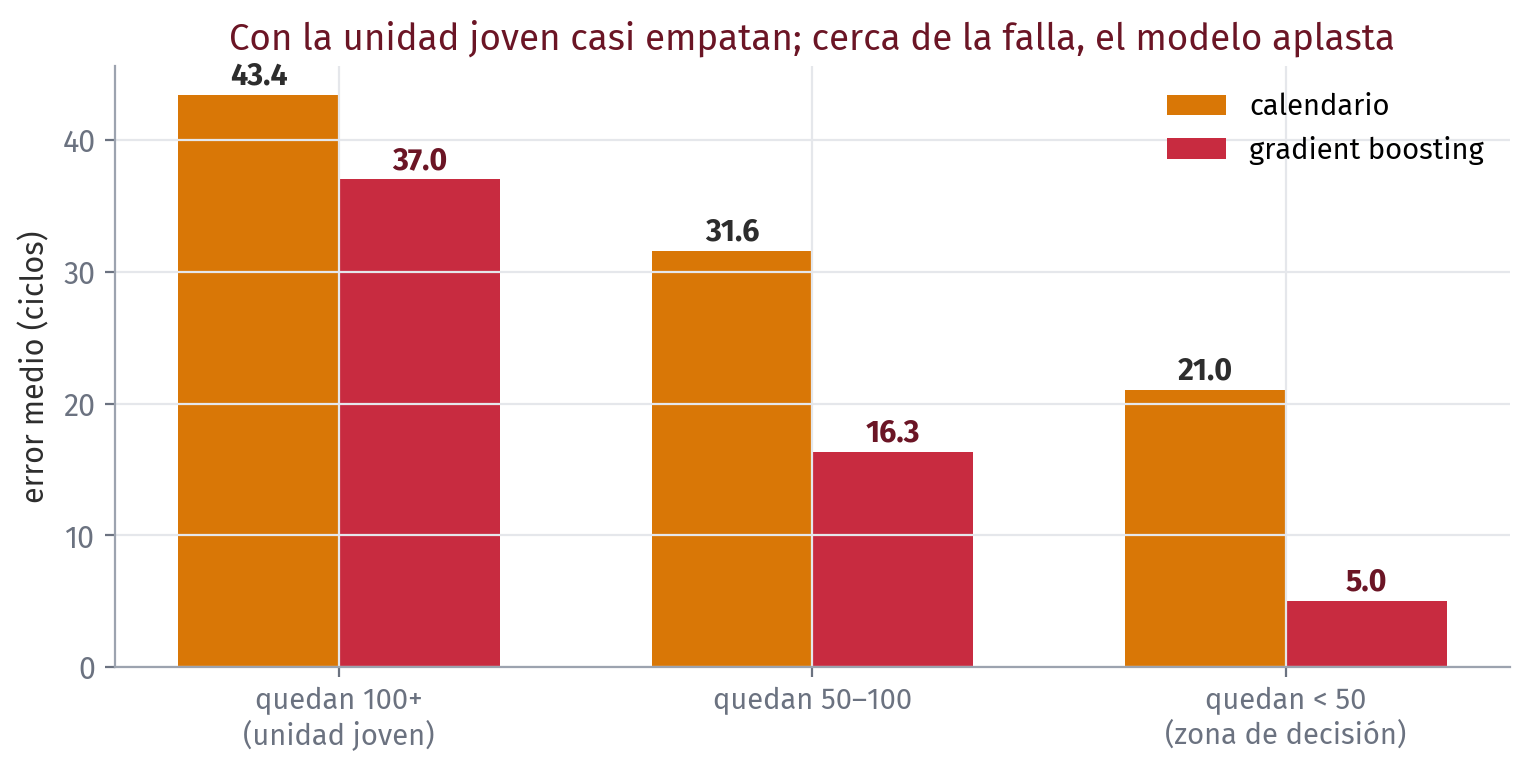
\includegraphics[height=0.56\textheight]{fig_zona.png}
  \end{center}
  \vspace{-2pt}
  {\footnotesize\color{textMuted}
   Partido el error por cuánta vida quedaba: con la unidad \textbf{joven},
   modelo y calendario casi empatan (37 vs 43). Pero cuando quedan menos
   de 50 ciclos --- \textbf{justo cuando se decide pedir el equipo} --- el
   calendario yerra por 21 y el modelo por \textbf{5}. La plata vive ahí.}
\end{frame}

\begin{frame}[shrink=20]{Una Unidad Vista de Cerca}
  \vspace{-6pt}
  \begin{center}
    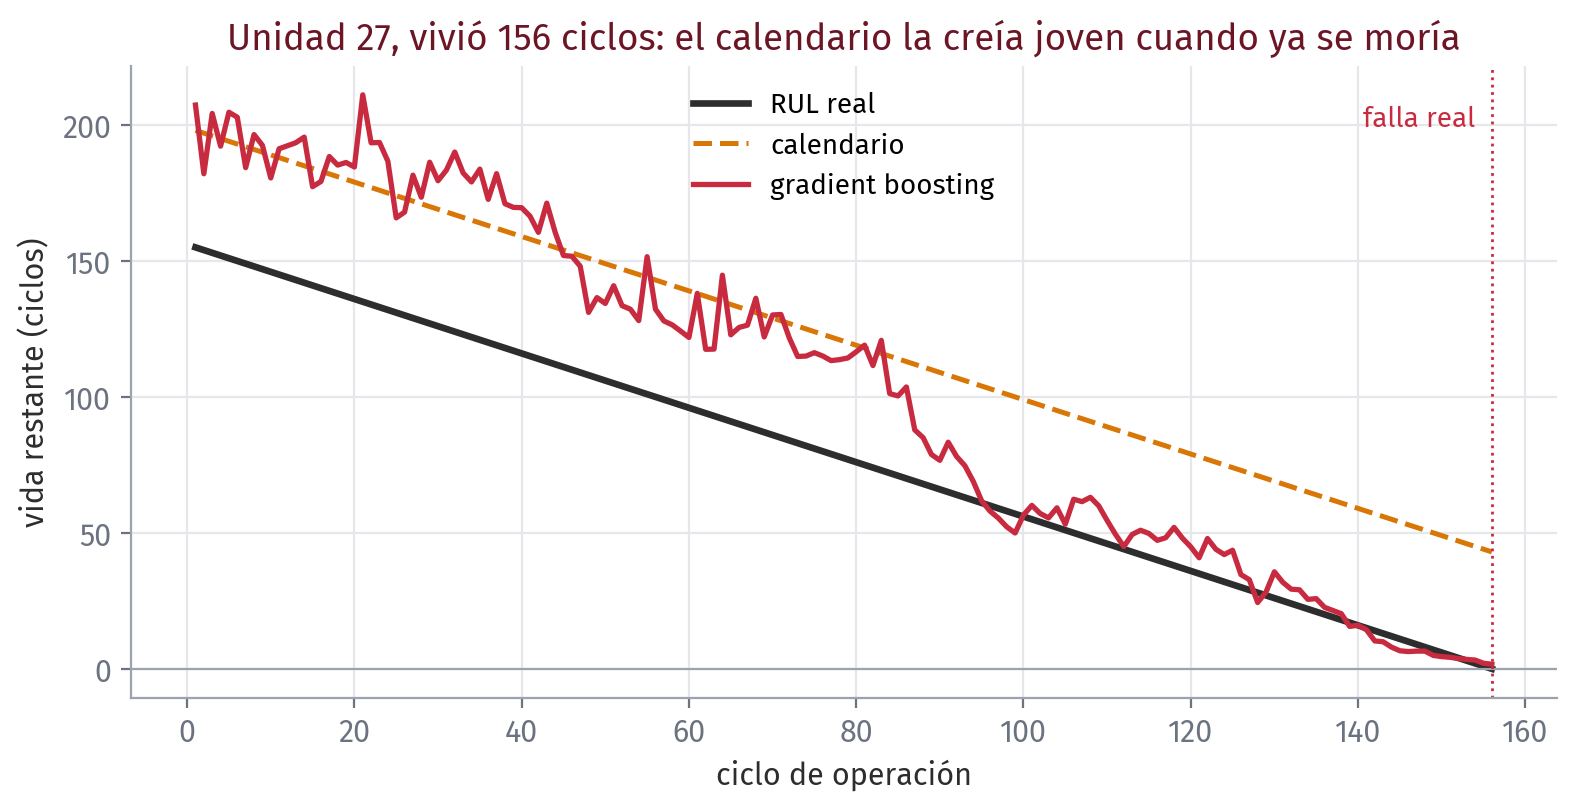
\includegraphics[height=0.56\textheight]{fig_unidad.png}
  \end{center}
  \vspace{-2pt}
  {\footnotesize\color{textMuted}
   La unidad 27 vivió \textbf{156 ciclos} --- de las cortas. El calendario
   (199 $-$ edad) la creía con 43 ciclos de vida \textbf{el día que murió}.
   El modelo la ve degradarse y \textbf{dobla hacia cero con ella}. Esta
   lámina es la clase entera en una figura.}
\end{frame}

\begin{frame}[shrink=8]{El Resultado Negativo de Hoy: la Unidad Joven}
  \vspace{2pt}
  \begin{tcolorbox}[colback=arcaGray, colframe=arcaRed, boxrule=0pt,
    leftrule=4pt, arc=3pt, left=10pt, right=10pt, top=8pt, bottom=8pt]
    {\normalsize\color{arcaDark}\bfseries
     Mientras la máquina está sana, el modelo NO sabe más que el
     calendario.}\\[6pt]
    {\footnotesize\color{textMuted}
     Con 100+ ciclos por delante los sensores todavía no muestran
     degradación --- y sin huella que leer, no hay nada que aprender:
     37 vs 43 ciclos de error, casi empate.}
  \end{tcolorbox}
  \vspace{9pt}
  {\footnotesize\color{textMuted}
   ¿Por qué esto es una \emph{buena} noticia? Porque delata cómo funciona
   de verdad: \textbf{el modelo no adivina el futuro --- reconoce la
   degradación presente y la proyecta}. Cuando no hay degradación, no
   promete nada.}
  \vspace{7pt}

  {\footnotesize\color{arcaDark}\bfseries\itshape
   Vacuna para la vida profesional: si un proveedor les ofrece predecir
   fallas «con seis meses de anticipación» en equipos sin degradación
   observable\ldots{} ya saben qué preguntarle.}
\end{frame}
% ═════════════════════════════════════════════════════════════════════════════
\sectionframe{El Porqué y el Precio}{Shapley para explicar cada pronóstico, y dólares para elegir la política \\[6pt] \normalsize 70 -- 95 min}
% ═════════════════════════════════════════════════════════════════════════════

\begin{frame}[shrink=8]{Un Pronóstico Sin Porqué No Se Firma}
  \vspace{2pt}
  {\footnotesize\color{textMuted}
  El modelo dice: \emph{«a la unidad 23 le quedan 43 ciclos»}. El
  supervisor que tiene que pedir el equipo va a hacer \textbf{una sola
  pregunta}: \emph{¿por qué?} Y hay dos maneras de responderla:}
  \vspace{8pt}
  \begin{columns}[T]
    \begin{column}{0.48\textwidth}
      \begin{tcolorbox}[colback=arcaGray, colframe=arcaDark, boxrule=0pt, leftrule=3pt,
        arc=3pt, left=8pt, right=8pt, top=5pt, bottom=5pt]
        {\scriptsize\color{arcaDark}\bfseries\faGlobe\hspace{4pt}GLOBAL:
         ¿en qué se fija el modelo?}\\[5pt]
        {\scriptsize\color{textMuted}
         En general, en toda la flota. Ya la conocen: es la
         \textbf{importancia por permutación} de la C3 --- desordenar una
         columna y medir cuánto duele.}
      \end{tcolorbox}
    \end{column}
    \begin{column}{0.48\textwidth}
      \begin{tcolorbox}[colback=arcaGray, colframe=arcaRed, boxrule=0pt, leftrule=3pt,
        arc=3pt, left=8pt, right=8pt, top=5pt, bottom=5pt]
        {\scriptsize\color{arcaRed}\bfseries\faSearchLocation\hspace{4pt}LOCAL:
         ¿por qué ESTE número, HOY?}\\[5pt]
        {\scriptsize\color{textMuted}
         Para \emph{esta} unidad, en \emph{esta} foto. Es la pregunta de
         la orden de trabajo --- y la nueva de hoy. La responde un señor
         llamado \textbf{Shapley}.}
      \end{tcolorbox}
    \end{column}
  \end{columns}
  \vspace{8pt}
  {\scriptsize\color{arcaDark}\itshape
   La global sirve para confiar en el modelo. La local sirve para firmar
   \textbf{una} decisión. Hacen falta las dos.}
\end{frame}

\begin{frame}[shrink=16]{Shapley: Repartir el Crédito de una Jugada}
  \vspace{2pt}
  {\footnotesize\color{textMuted}
  Lloyd Shapley (Nobel de economía 2012) resolvió un problema de juegos en
  equipo que es \emph{exactamente} el nuestro:}
  \vspace{7pt}
  \begin{tcolorbox}[colback=arcaGray, colframe=arcaRed, boxrule=0pt,
    leftrule=4pt, arc=3pt, left=10pt, right=10pt, top=7pt, bottom=7pt]
    {\footnotesize\color{arcaDark}
     Un equipo ganó un premio. ¿Cómo repartirlo \textbf{justo} entre los
     jugadores? Respuesta: midiendo cuánto cambia el resultado
     \textbf{con y sin cada jugador}, en todas las alineaciones posibles,
     y promediando.}
  \end{tcolorbox}
  \vspace{8pt}
  {\footnotesize\color{textMuted}
  Traducido a hoy:
  \begin{itemize}\setlength{\itemsep}{6pt}
    \item[{\color{arcaRed}\scriptsize\faArrowRight}]
      El «premio» es la \textbf{distancia} entre el pronóstico promedio de
      la flota y el pronóstico de esta unidad
    \item[{\color{arcaRed}\scriptsize\faArrowRight}]
      Los «jugadores» son las \textbf{46 columnas}: cada una recibe su
      pedazo del empuje, en ciclos, con signo
    \item[{\color{arcaRed}\scriptsize\faArrowRight}]
      Para modelos de árboles esto se calcula \textbf{exacto y rápido}
      (TreeSHAP) --- por eso hoy es el estándar de la industria
  \end{itemize}}
  \vspace{5pt}
  {\scriptsize\color{arcaDark}\itshape
   En código: \texttt{shap.TreeExplainer(modelo)}. Dos líneas. Lo difícil
   --- como siempre --- es leerlo bien.}
\end{frame}

\begin{frame}[shrink=20]{El Porqué de la Unidad 23, Pieza por Pieza}
  \vspace{-6pt}
  \begin{center}
    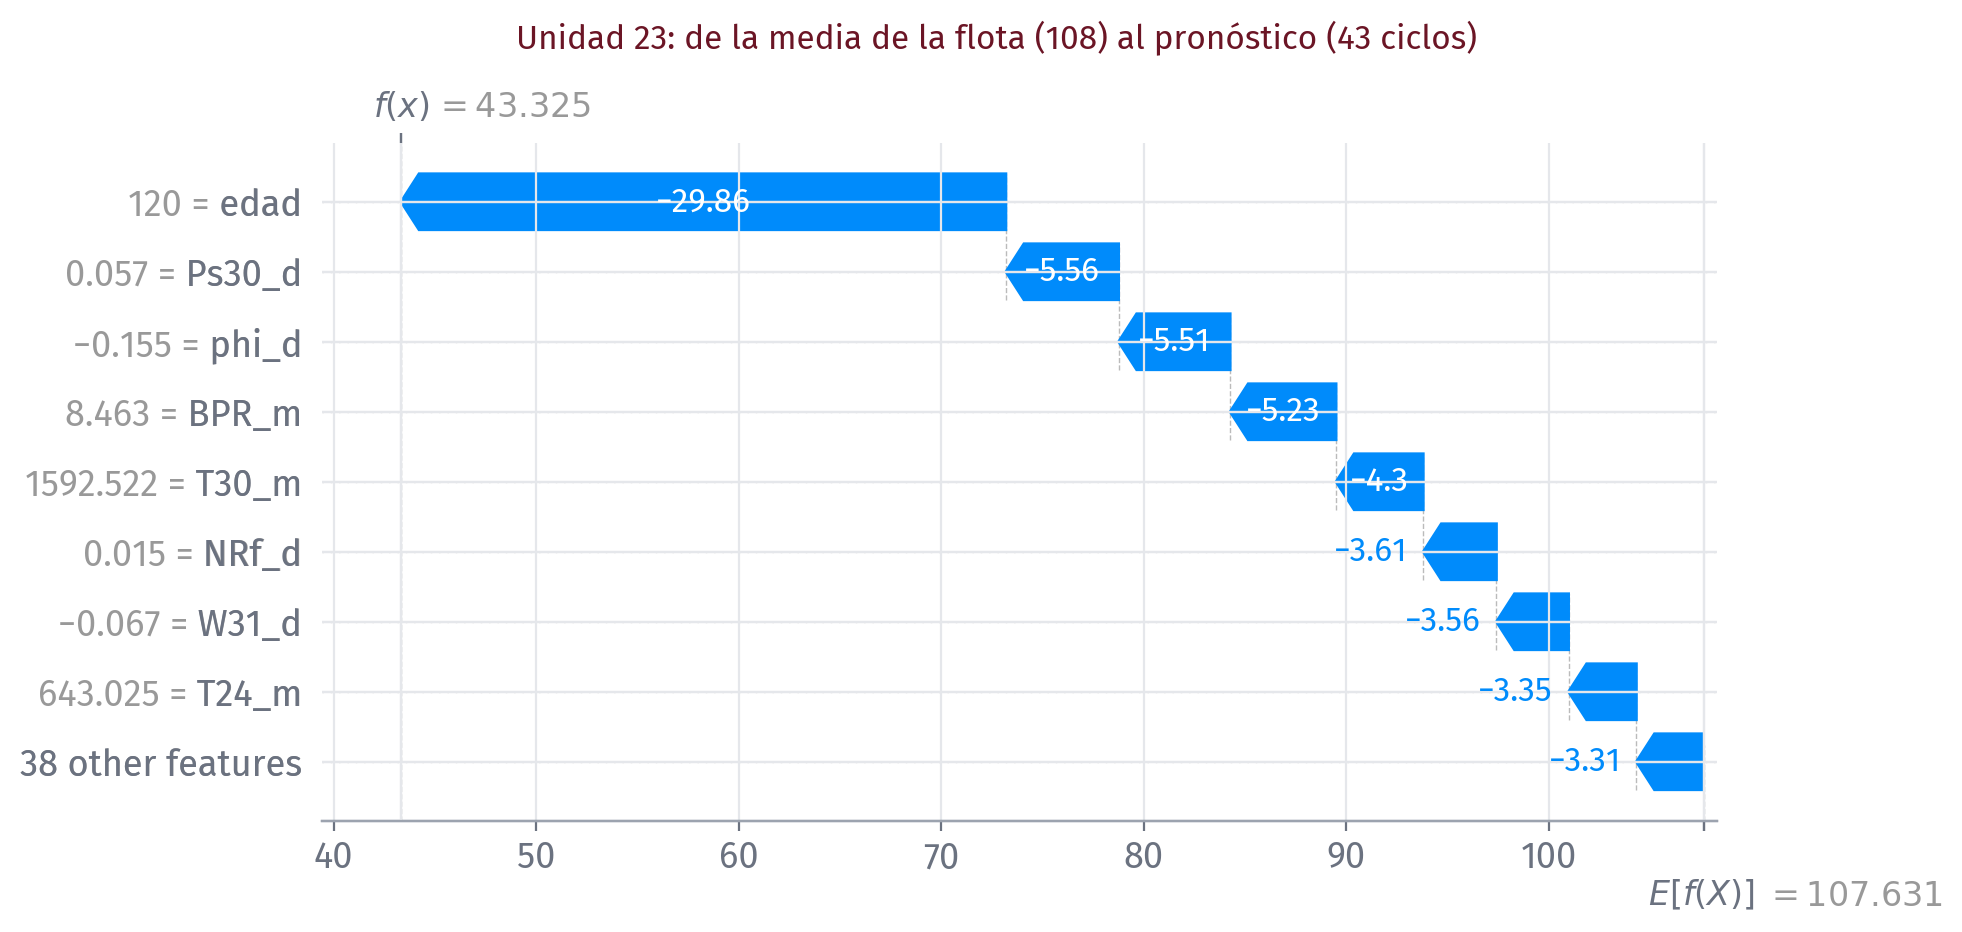
\includegraphics[height=0.56\textheight]{fig_shap_local.png}
  \end{center}
  \vspace{-2pt}
  {\footnotesize\color{textMuted}
   Se lee de abajo hacia arriba: la flota promedia \textbf{108} ciclos de
   RUL; la edad de esta unidad empuja $-$30; la presión del compresor
   cayendo (\texttt{Ps30\_d}), el consumo torciéndose (\texttt{phi\_d}) y
   el resto suman su parte\ldots{} pronóstico final: \textbf{43}. El RUL
   real era \textbf{48}. Esto ya es un párrafo de orden de trabajo.}
\end{frame}

\begin{frame}[shrink=20]{La Flota Entera, Repartida por Shapley}
  \vspace{-6pt}
  \begin{center}
    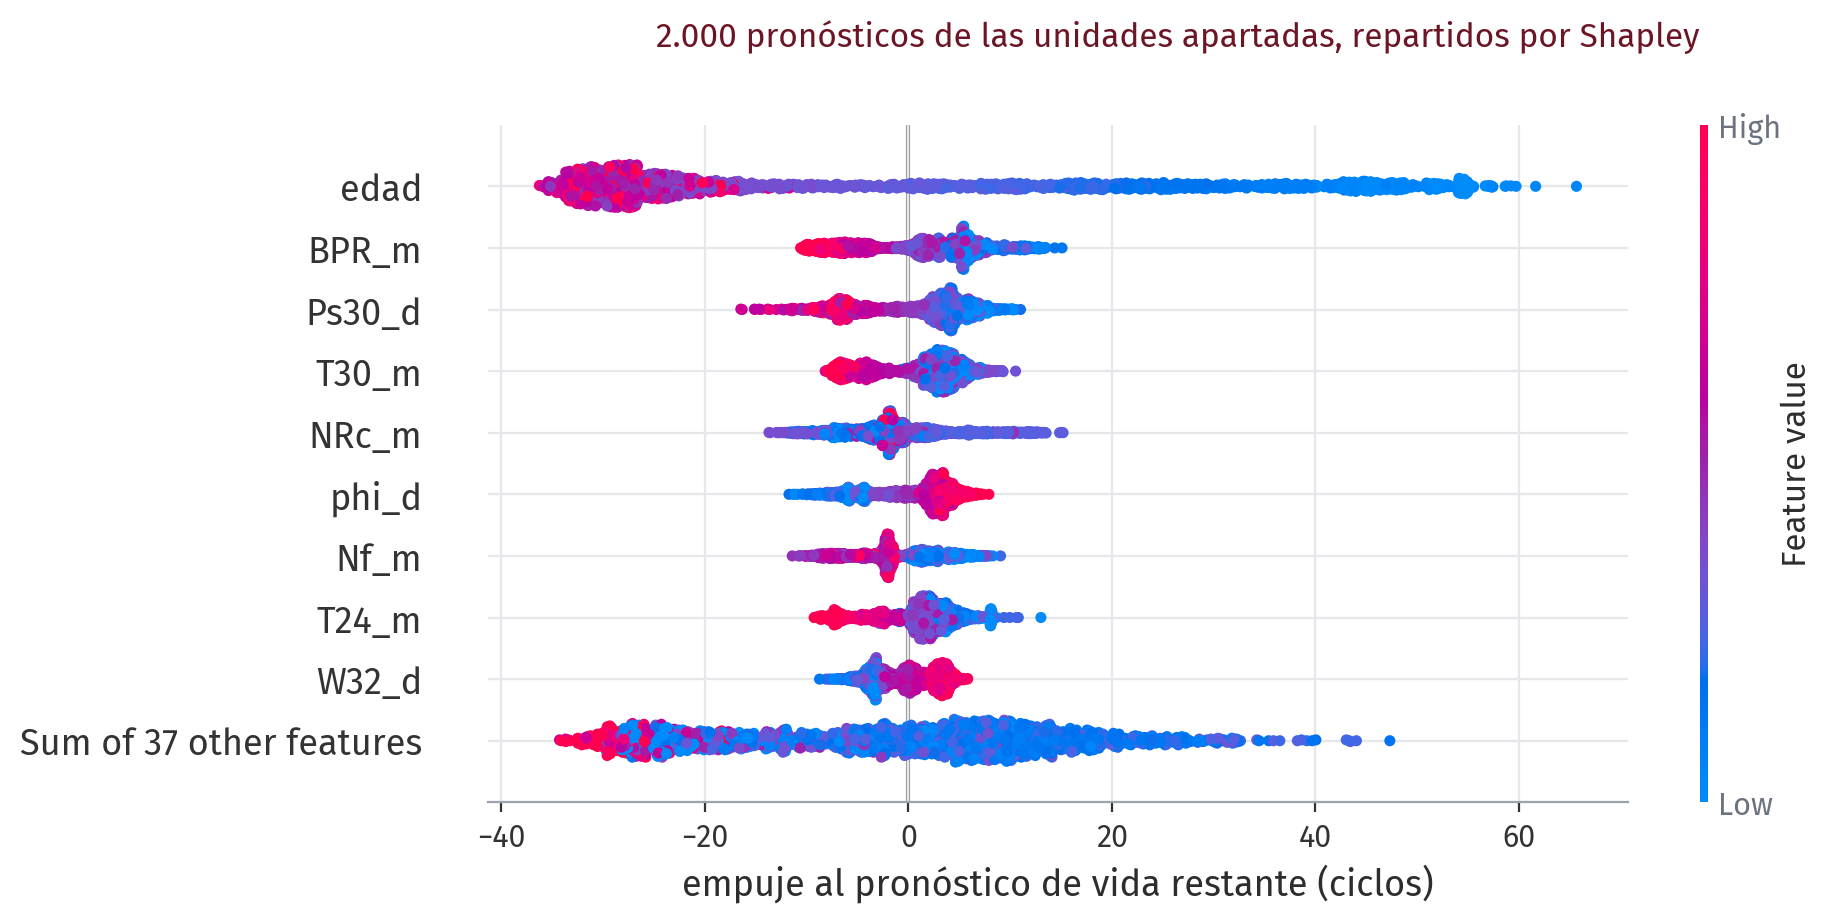
\includegraphics[height=0.56\textheight]{fig_shap_global.png}
  \end{center}
  \vspace{-2pt}
  {\footnotesize\color{textMuted}
   Cada punto es un pronóstico; el color, el valor del sensor. Léanlo como
   ingenieros: \texttt{BPR} alto (rojo) empuja la vida \textbf{hacia
   abajo}, \texttt{Ps30} cayendo también. El modelo redescubrió la
   termodinámica de la degradación --- \textbf{sin que nadie se la
   contara}.}
\end{frame}

\begin{frame}[shrink=22]{La Letra Chica de Shapley (Léanla Siempre)}
  \vspace{2pt}
  \begin{tcolorbox}[colback=arcaGray, colframe=arcaRed, boxrule=0pt,
    leftrule=4pt, arc=3pt, left=10pt, right=10pt, top=7pt, bottom=7pt]
    {\footnotesize\color{arcaDark}\bfseries
     Shapley reparte el pronóstico DEL MODELO. No reparte la culpa
     física.}\\[5pt]
    {\footnotesize\color{textMuted}
     Si dos sensores cuentan la misma historia (y en una máquina
     degradándose, casi todos la cuentan), se \textbf{roban crédito}
     entre sí. El reparto es fiel al modelo, no al mecanismo.}
  \end{tcolorbox}
  \vspace{8pt}
  {\footnotesize\color{textMuted}
  La prueba, con nuestros propios números:
  \begin{itemize}\setlength{\itemsep}{6pt}
    \item[{\color{arcaRed}\scriptsize\faArrowRight}]
      En el waterfall, la \textbf{edad} se llevó $-$30 ciclos: el pedazo
      más grande por lejos
    \item[{\color{arcaRed}\scriptsize\faArrowRight}]
      Pero cuando \textbf{le quitamos la edad} al modelo y lo
      reentrenamos\ldots{} el error casi no cambió: 24,2 contra 24,4
    \item[{\color{arcaRed}\scriptsize\faArrowRight}]
      Conclusión: la información de la edad \textbf{también vive en los
      sensores} (una máquina vieja \emph{se ve} vieja). Shapley le dio el
      crédito a la edad porque el modelo la usó primero --- no porque
      fuera imprescindible
  \end{itemize}}
  \vspace{5pt}
  {\scriptsize\color{arcaDark}\itshape
   Ese experimento se llama \textbf{ablación}: quitar una pieza y medir.
   Shapley les dice qué usó el modelo; la ablación, qué necesitaba. Con
   las dos, la explicación aguanta una reunión hostil.}
\end{frame}

\begin{frame}[shrink=6]{El Error Tiene Dirección, y los Precios También}
  \vspace{-6pt}
  \begin{center}
    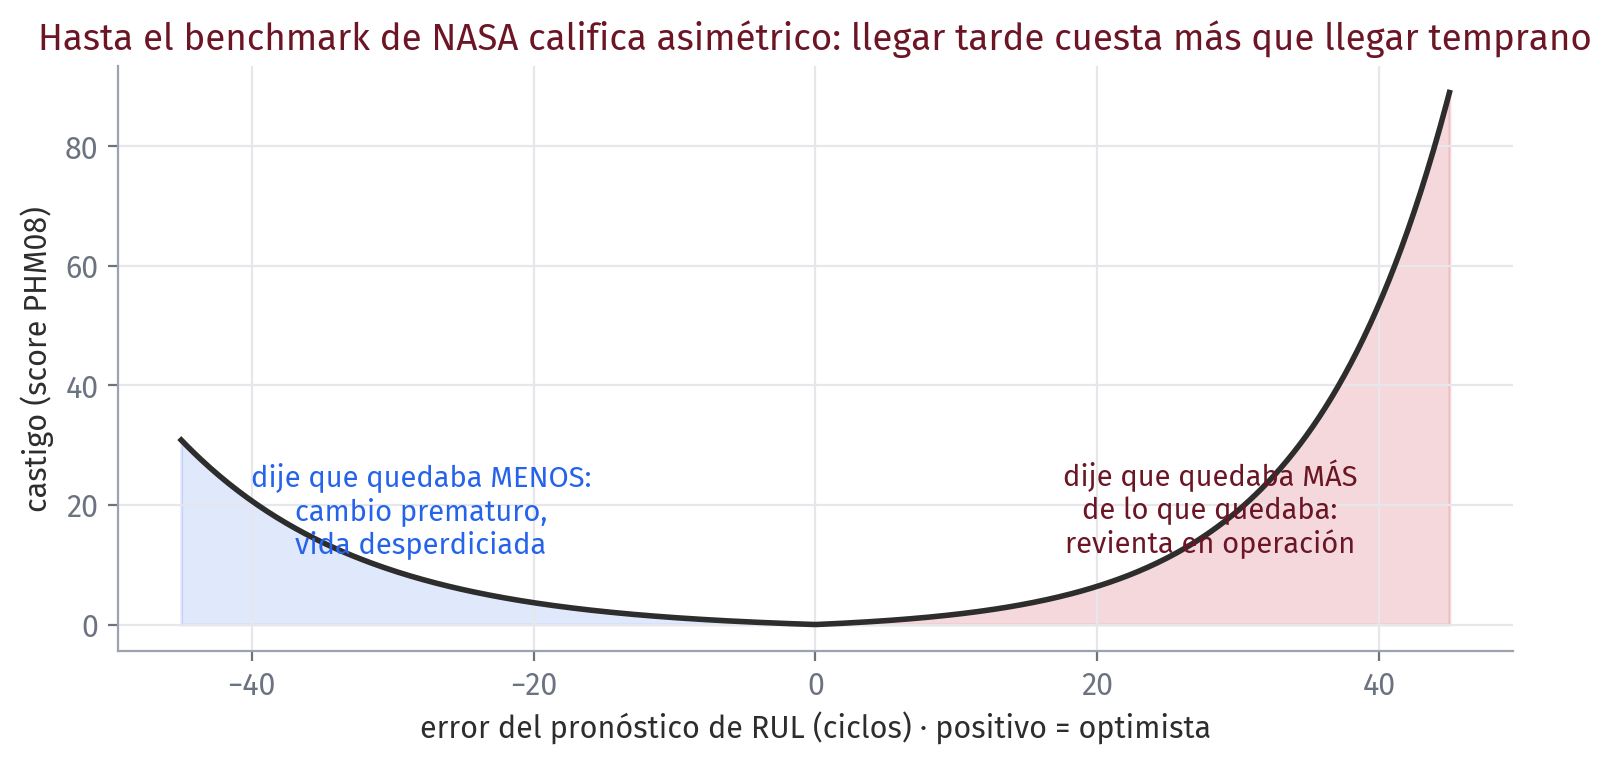
\includegraphics[height=0.52\textheight]{fig_asimetria.png}
  \end{center}
  \vspace{-2pt}
  {\footnotesize\color{textMuted}
   Decir «le quedan 60» cuando quedaban 20 $\rightarrow$ bomba muerta
   esperando equipo: \textbf{1,5 MUSD}. Decir «le quedan 20» cuando
   quedaban 60 $\rightarrow$ vida desperdiciada: mucho más barato. Hasta
   el examen oficial del PHM08 castiga así, con exponenciales asimétricas.
   \textbf{El P50 ignora esto. La decisión no puede.}}
\end{frame}

\begin{frame}[shrink=20]{No Se Opera con el Promedio: el P10}
  \vspace{-6pt}
  \begin{center}
    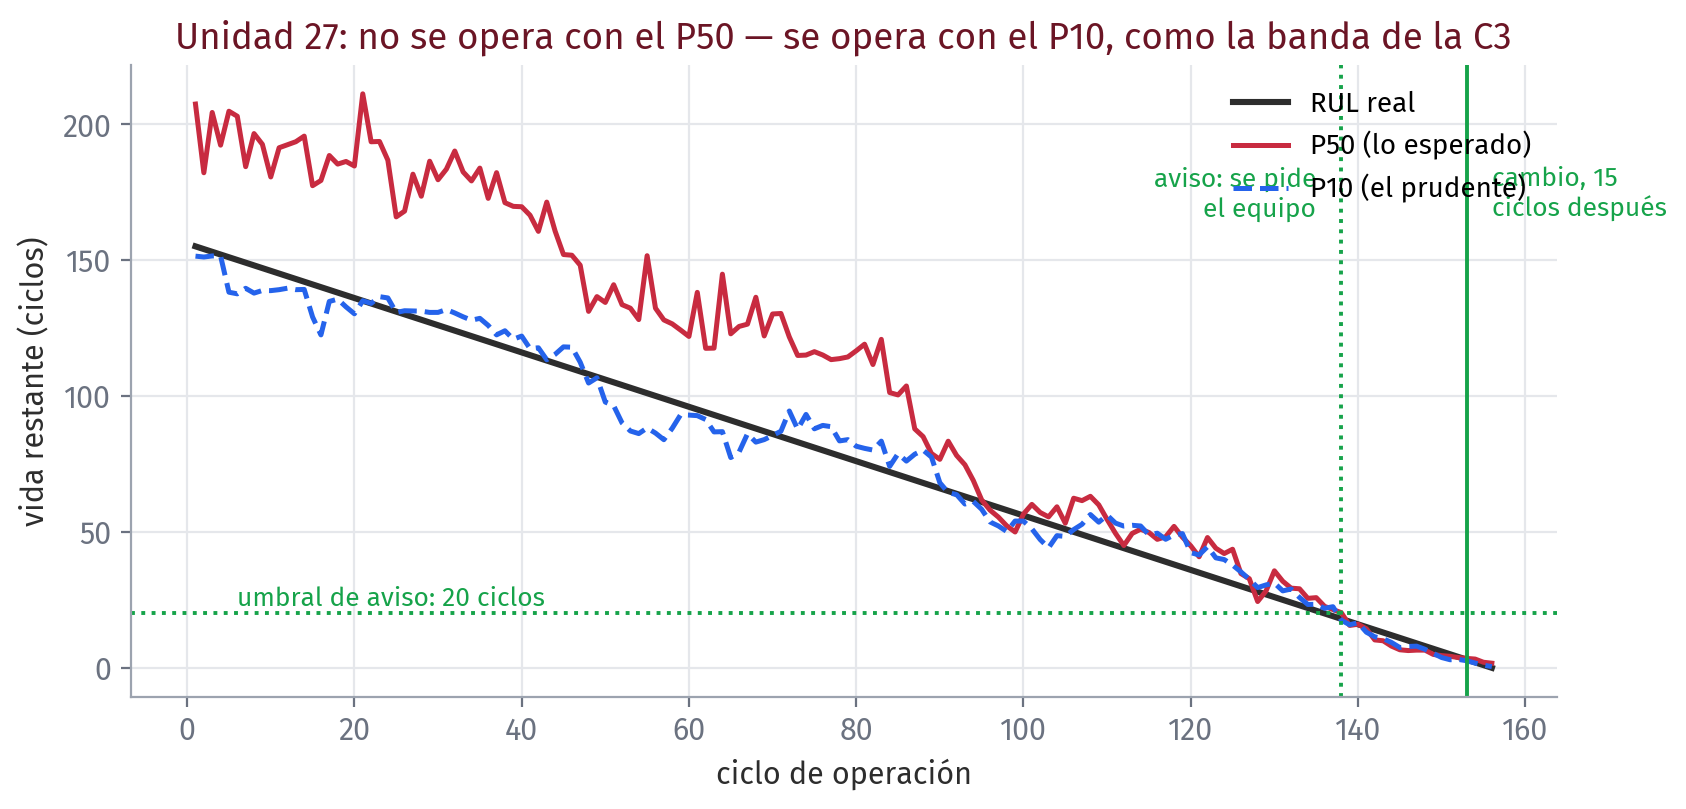
\includegraphics[height=0.54\textheight]{fig_cuantiles.png}
  \end{center}
  \vspace{-2pt}
  {\footnotesize\color{textMuted}
   El mismo boosting, entrenado con pérdida de cuantil
   (\texttt{loss="quantile"}): el \textbf{P10} es la versión prudente
   del reloj --- «con 90 \% de confianza, le queda \emph{al menos}
   esto». Auditado en las 25 apartadas cumplió \textbf{83 \%} contra 90
   nominal: un poco optimista, y se declara --- igual que auditamos la
   banda en la C3.}
\end{frame}

\begin{frame}[shrink=8]{La Regla de Decisión, Completa en Tres Líneas}
  \vspace{2pt}
  \begin{tcolorbox}[colback=arcaGray, colframe=arcaRed, boxrule=0pt,
    leftrule=4pt, arc=3pt, left=10pt, right=10pt, top=8pt, bottom=8pt]
    {\normalsize\color{arcaDark}
     \textbf{1.} Cada ciclo, mirar el \textbf{P10} del RUL de cada
     unidad.\\[5pt]
     \textbf{2.} Si baja de \textbf{20 ciclos} $\rightarrow$ pedir el
     equipo hoy.\\[5pt]
     \textbf{3.} El cambio ocurre \textbf{15 ciclos después} (lo que
     tarda la movilización).}
  \end{tcolorbox}
  \vspace{9pt}
  {\footnotesize\color{textMuted}
   Cada número tiene dueño: el \textbf{15} es de logística (cuánto tarda
   el equipo en llegar --- pregúntenle a operaciones, no al modelo). El
   \textbf{20} es el 15 más un colchón que paga la imperfección del P10.
   Y el \textbf{P10} --- no el P50 --- es porque el error hacia arriba
   cuesta 5 veces más.}
  \vspace{6pt}

  {\footnotesize\color{arcaDark}\bfseries\itshape
   Noten qué pasó: la estadística puso el pronóstico, la logística puso
   el 15, y finanzas puso el P10. Una regla de decisión de verdad
   siempre tiene esas tres firmas.}
\end{frame}

\begin{frame}[shrink=20]{Las Cuatro Políticas, en Dólares}
  \vspace{-6pt}
  \begin{center}
    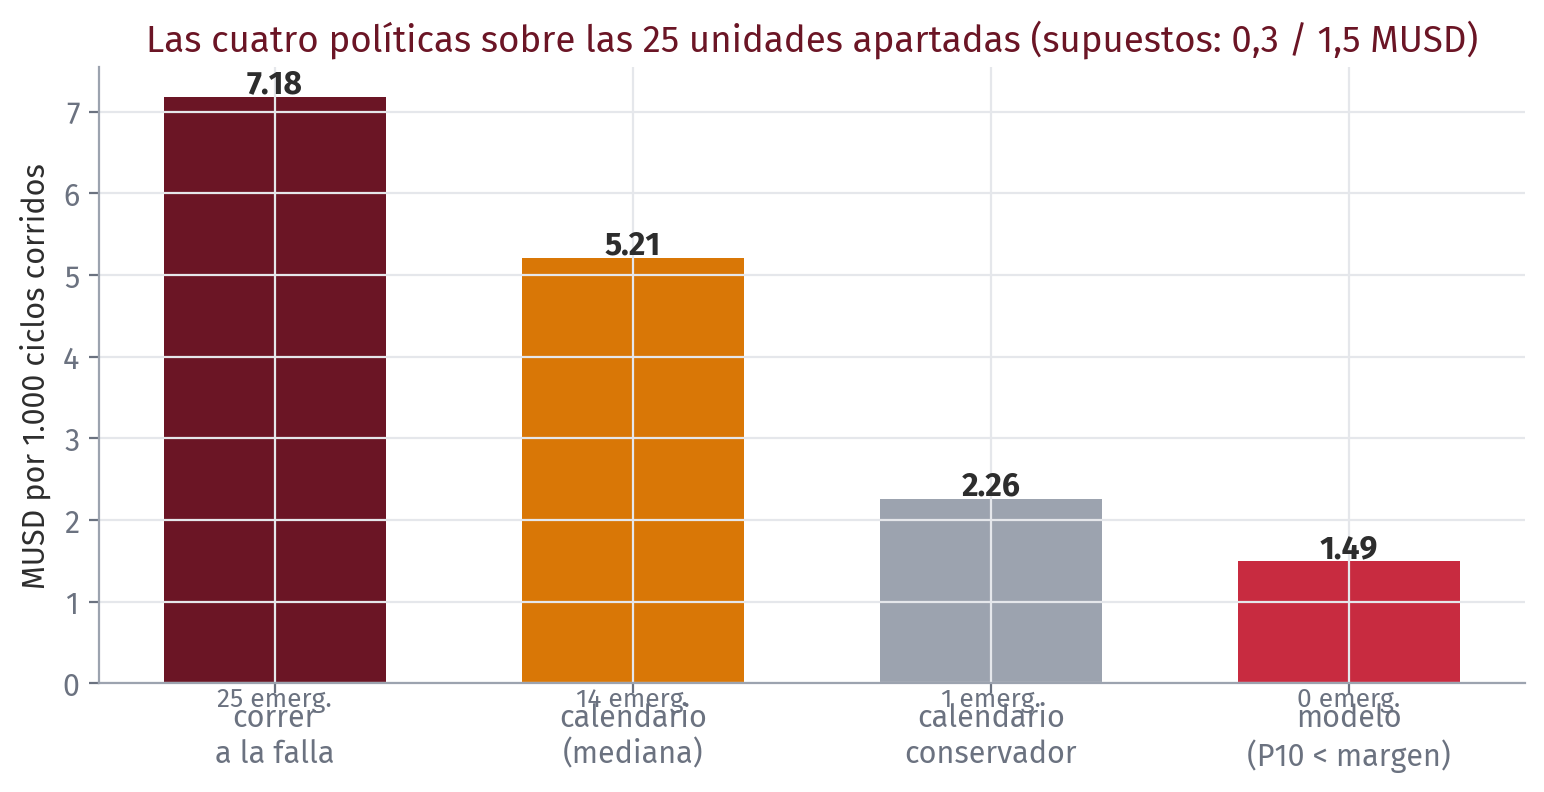
\includegraphics[height=0.54\textheight]{fig_politicas.png}
  \end{center}
  \vspace{-2pt}
  {\footnotesize\color{textMuted}
   Sobre las 25 unidades apartadas, vida completa, mismos supuestos:
   correr a la falla cuesta \textbf{7,18}; el calendario común, 5,21
   (¡14 emergencias!); el calendario conservador se salva de las
   emergencias pero \textbf{bota 41 ciclos} de vida por unidad: 2,26. El
   modelo: \textbf{0 emergencias, 5 ciclos botados, 1,49} --- un
   \textbf{34 \% más barato} que el mejor calendario posible.}
\end{frame}

\begin{frame}[shrink=20]{El Entregable: la Lista del Mes}
  \vspace{-6pt}
  \begin{center}
    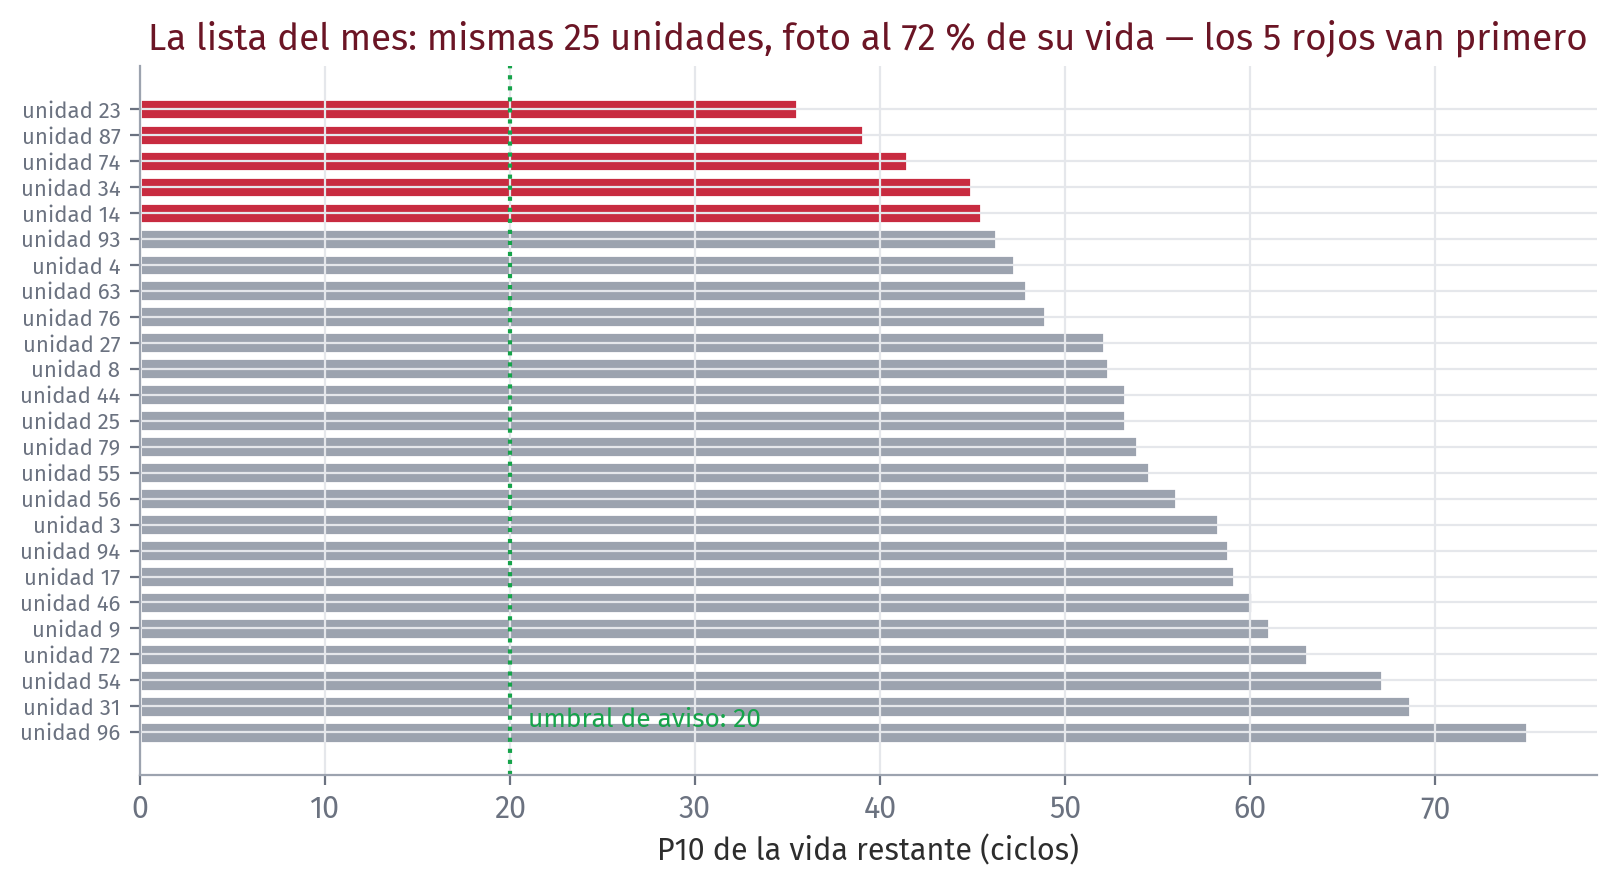
\includegraphics[height=0.56\textheight]{fig_lista.png}
  \end{center}
  \vspace{-2pt}
  {\footnotesize\color{textMuted}
   La foto de hoy de la flota, ordenada por el P10. Los cinco rojos van
   primero --- y gracias a Shapley, \textbf{cada uno lleva su porqué}
   («Ps30 cayendo, consumo subiendo») en la orden de trabajo. Esto es lo
   que se firma. El resto de la flota: a seguir corriendo.}
\end{frame}

\begin{frame}[shrink=8]{Cómo Reportarlo al que Decide}
  \vspace{-4pt}
  \begin{columns}[T]
    \begin{column}{0.48\textwidth}
      \begin{tcolorbox}[colback=arcaGray, colframe=arcaRed, boxrule=0pt, leftrule=3pt,
        arc=3pt, left=6pt, right=6pt, top=5pt, bottom=5pt]
        {\scriptsize\color{arcaRed}\bfseries\faBan\hspace{4pt}ASÍ NO}\\[5pt]
        {\scriptsize\color{textMuted}\itshape
         «Entrenamos un HistGradientBoostingRegressor con malla de
         hiperparámetros por GroupKFold y logramos un MAE de 24,4 contra
         35,2 del baseline.»}\\[5pt]
        {\scriptsize\color{textMuted}
         Todo cierto. Nada decidible.}
      \end{tcolorbox}
    \end{column}
    \begin{column}{0.48\textwidth}
      \begin{tcolorbox}[colback=arcaGray, colframe=codeGreen, boxrule=0pt, leftrule=3pt,
        arc=3pt, left=6pt, right=6pt, top=5pt, bottom=5pt]
        {\scriptsize\color{codeGreen}\bfseries\faCheck\hspace{4pt}ASÍ SÍ}\\[5pt]
        {\scriptsize\color{textMuted}\itshape
         «Con los sensores que ya tenemos, el plan de cambios pasa de 14
         fallas sorpresa a \textbf{cero}, botando 5 ciclos de vida por
         bomba en vez de 41. Es un \textbf{34 \% menos} de costo de
         mantenimiento por ciclo corrido que el mejor calendario.\\[4pt]
         La lista de este mes tiene 5 bombas, cada una con su motivo.»}
      \end{tcolorbox}
    \end{column}
  \end{columns}
  \vspace{8pt}
  {\footnotesize\color{arcaDark}\itshape
   La versión de la derecha se puede llevar a un comité de presupuesto.
   Y cada número de ese párrafo salió de una lámina de hoy --- ninguno
   es de fe.}
\end{frame}

% ═════════════════════════════════════════════════════════════════════════════
\sectionframe{Su Turno}{Otro costo, otra decisión --- el mismo modelo \\[6pt] \normalsize 95 -- 118 min}
% ═════════════════════════════════════════════════════════════════════════════

\begin{frame}[shrink=22]{Su Turno: Firmen Su Propia Regla \hfill {\normalsize\color{arcaRed}\faClock\hspace{4pt}20 min}}
  \vspace{-2pt}
  {\footnotesize\color{textMuted}
  En el cuaderno está todo montado: el modelo entrenado, el P10 por
  unidad, y la simulación de políticas \textbf{como función}. Ustedes
  operan un campo distinto al de la clase:}
  \vspace{6pt}
  \begin{tcolorbox}[colback=arcaGray, colframe=arcaDark, boxrule=0pt, leftrule=3pt,
    arc=3pt, left=8pt, right=8pt, top=5pt, bottom=5pt]
    {\scriptsize\color{arcaDark}\bfseries EL ESCENARIO B --- CAMPO EN TIERRA}\\[4pt]
    {\scriptsize\color{textMuted}
     Cambio programado: \textbf{0,08 MUSD} · Falla en operación:
     \textbf{0,16 MUSD} (hay equipo cerca: la sorpresa solo cuesta el
     doble, no cinco veces). La movilización tarda \textbf{5} ciclos.}
  \end{tcolorbox}
  \vspace{6pt}
  {\footnotesize\color{textMuted}
  \begin{itemize}\setlength{\itemsep}{5pt}
    \item[{\color{arcaRed}\scriptsize 1.}]
      Corran las cuatro políticas con \emph{sus} costos. ¿Sigue ganando
      el modelo? ¿Por cuánto?
    \item[{\color{arcaRed}\scriptsize 2.}]
      Ajusten el umbral de aviso (prueben 10, 20, 30) y quédense con el
      más barato. ¿Les dio distinto que a la clase? ¿Por qué?
    \item[{\color{arcaRed}\scriptsize 3.}]
      Escriban el párrafo «Así Sí» para \emph{su} gerente, con sus
      números
  \end{itemize}}
  \vspace{5pt}
  {\scriptsize\color{arcaDark}\itshape
   Pista de la trampa: cuando la sorpresa cuesta casi lo mismo que el
   plan, la prudencia deja de ser gratis. No busquen la respuesta de la
   clase: busquen la de su campo.}
\end{frame}

\begin{frame}[shrink=8]{Lo Que Deben Encontrar (No Lean Antes de Intentar)}
  \vspace{2pt}
  {\footnotesize\color{textMuted}
  El punto andragógico del ejercicio, dicho después de sudarlo:}
  \vspace{8pt}
  \begin{tcolorbox}[colback=arcaGray, colframe=arcaRed, boxrule=0pt,
    leftrule=4pt, arc=3pt, left=10pt, right=10pt, top=8pt, bottom=8pt]
    {\normalsize\color{arcaDark}\bfseries
     Mismo modelo, mismos pronósticos, otra estructura de costos
     $\rightarrow$ OTRA política óptima.}\\[6pt]
    {\footnotesize\color{textMuted}
     Con la falla a solo 2$\times$, esperar más y tolerar alguna
     emergencia puede salir más barato que ser prudente. El umbral óptimo
     se corre, y hasta el calendario puede volver a ser competitivo.}
  \end{tcolorbox}
  \vspace{9pt}
  {\footnotesize\color{arcaDark}\itshape
   La decisión nunca estuvo dentro del modelo: estuvo en los costos.
   El modelo pone el pronóstico; el negocio pone el umbral. Quien
   entiende eso no vuelve a pedir «el mejor modelo» --- pide \textbf{el
   mejor sistema de decisión}.}
\end{frame}

% ═════════════════════════════════════════════════════════════════════════════
\sectionframe{Cierre}{}
% ═════════════════════════════════════════════════════════════════════════════

\begin{frame}[shrink=10]{Lo Que Aprendimos Hoy}
  \vspace{-4pt}
  {\scriptsize
  \begin{center}
  \begin{tabular}{p{0.44\textwidth}p{0.46\textwidth}}
    \toprule
    \textbf{lo que vimos} & \textbf{lo que decidimos con eso} \\
    \midrule
    Vidas de 128 a 362 ciclos en máquinas gemelas & El calendario ingenuo pierde: 14 sorpresas de 25 \\[3pt]
    La degradación deja huella en los sensores & Convertirla en RUL: el reloj que corre hacia atrás \\[3pt]
    Gradient boosting: la cadena que corrige & Error de 5 ciclos en la zona de decisión (4$\times$ mejor) \\[3pt]
    La malla afinó con método (GroupKFold) & \ldots{}y compró 0,2 ciclos: afinar al final, no primero \\[3pt]
    Shapley reparte el porqué de cada pronóstico & Órdenes de trabajo con motivo --- y con letra chica \\[3pt]
    El P10 y la regla de los tres números & 0 emergencias y 34 \% menos costo que el mejor calendario \\
    \bottomrule
  \end{tabular}
  \end{center}}
  \vspace{6pt}
  {\scriptsize\color{arcaDark}\itshape
   Y el arco del módulo quedó cerrado: la C2 detecta, la C3 acota, la C4
   prioriza, la C5 \textbf{decide}.}
\end{frame}

\begin{frame}[shrink=8]{Los Resultados Negativos de Hoy}
  \vspace{2pt}
  {\footnotesize\color{textMuted}
  Como todas las clases de este módulo: lo que \textbf{no} funcionó,
  dicho en voz alta.}
  \vspace{8pt}
  {\footnotesize
    \begin{itemize}\setlength{\itemsep}{9pt}
    \item[{\color{arcaRed}\faTimesCircle}]
      \textbf{Con la unidad joven, el modelo no sabe más que el
      calendario} (37 vs 43). Sin degradación visible no hay pronóstico
      fino --- el modelo proyecta el presente, no adivina el futuro.
    \item[{\color{arcaRed}\faTimesCircle}]
      \textbf{El afinado compró 0,2 ciclos.} La malla entera vive en 1,7
      ciclos de rango. Si esperaban magia de los hiperparámetros: no la
      hay --- la ganancia vivía en el modelo y los features.
    \item[{\color{arcaRed}\faTimesCircle}]
      \textbf{El P10 prometió 90 \% y cumplió 83 \%.} Igual que la banda
      de la C3 (76 contra 80): los cuantiles aprendidos tienden al
      optimismo, y por eso el umbral de aviso lleva colchón.
    \end{itemize}}
  \vspace{7pt}
  {\scriptsize\color{arcaDark}\itshape
   Tres limitaciones medidas y declaradas valen más que una demo
   perfecta. Esa es la diferencia entre una clase y un folleto.}
\end{frame}

\begin{frame}[shrink=8]{Si Se Llevan Una Sola Cosa}
  \vspace{6pt}
  \begin{tcolorbox}[colback=arcaGray, colframe=arcaRed, boxrule=0pt,
    leftrule=4pt, arc=3pt, left=12pt, right=12pt, top=10pt, bottom=10pt]
    {\large\color{arcaDark}\bfseries
     Un modelo no vale por su error promedio: vale por las decisiones
     que cambia.}\\[8pt]
    {\footnotesize\color{textMuted}
     El boosting le ganó al calendario por 11 ciclos de MAE --- y eso no
     convence a nadie. Le ganó por \textbf{14 emergencias evitadas y un
     34 \% del presupuesto de mantenimiento} --- y eso aprueba proyectos.
     La traducción del primero al segundo la hicieron el P10, un umbral
     con dueño y dos costos puestos a la vista. Esa traducción es el
     trabajo de ustedes.}
  \end{tcolorbox}
  \vspace{8pt}
  {\footnotesize\color{arcaDark}\itshape
   Y su hermana chica, para el día a día: cuando les presenten un modelo,
   pregunten primero \emph{«¿contra qué política vigente compite, y en
   qué unidades se mide la ganancia?»}. Si no hay respuesta, no hay
   proyecto.}
\end{frame}

\begin{frame}[shrink=24]{La Cuenta del Módulo, Como Se Prometió}
  \vspace{-2pt}
  \begin{tcolorbox}[colback=arcaGray, colframe=codeGreen, boxrule=0pt, leftrule=3pt,
    arc=3pt, left=8pt, right=8pt, top=5pt, bottom=5pt]
    {\scriptsize\color{codeGreen}\bfseries\faCheck\hspace{4pt}TEMARIO CONTRATADO: CUBIERTO EN ESTAS CINCO CLASES}\\[4pt]
    {\scriptsize\color{textMuted}
     \textbf{DCA probabilístico} (C3, con Arps pagado) ·
     \textbf{GOR y WOR} (C4) · \textbf{Breakthrough de agua} (C4) ·
     \textbf{Fallas de equipo de levantamiento} (C2: el método sobre un
     choke · C5: RUL y decisión, sobre turbomáquinas de NASA --- la
     sustitución de dato, declarada ambas veces) ·
     \textbf{Optimización de levantamiento artificial} (C5: cuándo
     intervenir cada unidad bajo costos --- dimensionamiento y gas lift
     quedan fuera) \\[3pt]
     \textbf{Las 3 prácticas comprometidas: entregadas} (series de
     tiempo C2 · WOR C4 · integración volumétrica + forecasting C3).}
  \end{tcolorbox}
  \vspace{6pt}
  \begin{tcolorbox}[colback=arcaGray, colframe=arcaRed, boxrule=0pt, leftrule=3pt,
    arc=3pt, left=8pt, right=8pt, top=5pt, bottom=5pt]
    {\scriptsize\color{arcaRed}\bfseries\faArrowCircleRight\hspace{4pt}DIFERIDO AL PROYECTO INTEGRADOR, EXPLÍCITAMENTE}\\[4pt]
    {\scriptsize\color{textMuted}
     Feature selection para \textbf{EOR} · \textbf{presión promedio} de
     yacimiento · análisis de \textbf{pruebas de presión} (DST, RFT,
     buildup) · \textbf{daño de formación}. En 10 horas, a la
     profundidad de este curso, no entraban --- y preferimos deberlas a
     fingirlas. Se retoman sobre los datos de ustedes.}
  \end{tcolorbox}
  \vspace{5pt}
  {\scriptsize\color{arcaDark}\itshape
   5 de 9 temas a fondo, 3 de 3 prácticas, y las deudas por escrito.
   Esa es la cuenta.}
\end{frame}

\begin{frame}[shrink=10]{Datos y Referencias}
  \vspace{4pt}
  {\footnotesize\color{textMuted}
  \begin{itemize}\setlength{\itemsep}{6pt}
    \item[{\color{arcaRed}\scriptsize\faDatabase}]
      \textbf{NASA C-MAPSS} --- \emph{Turbofan Engine Degradation
      Simulation Data Set}, Prognostics Center of Excellence, NASA Ames.
      Dominio público. Saxena, Goebel, Simon \& Eklund (2008),
      \emph{Damage Propagation Modeling\ldots}, PHM08.
    \item[{\color{arcaRed}\scriptsize\faBook}]
      \textbf{Lundberg \& Lee (2017)} --- \emph{A Unified Approach to
      Interpreting Model Predictions} (SHAP), NeurIPS. Y
      \textbf{Grinsztajn et al. (2022)} --- \emph{Why do tree-based
      models still outperform deep learning on tabular data?}, NeurIPS.
    \item[{\color{arcaRed}\scriptsize\faFileCode}]
      El CSV curado se construye con
      \texttt{modulo5-clase5/preparar\_datos.py}; las figuras y
      \textbf{todas} las cifras de estas láminas salen de
      \texttt{figuras.py}. Nada está escrito a mano.
  \end{itemize}}
  \vspace{7pt}
  {\scriptsize\color{arcaDark}\itshape
   Como siempre: clonan el repositorio, corren los dos scripts, y tiene
   que dar exactamente lo mismo. Si no da, es un error nuestro y queremos
   saberlo.}
\end{frame}

% ── GRACIAS ──────────────────────────────────────────────────────────────────
\begingroup
\setbeamertemplate{headline}{}
\setbeamertemplate{footline}{}
\setbeamertemplate{navigation symbols}{}
\begin{frame}[plain, noframenumbering]
  \begin{tikzpicture}[remember picture, overlay]
    \fill[arcaDark] (current page.south west) rectangle (current page.north east);
    \node[anchor=center, text=white, font=\Huge\bfseries]
      at ([yshift=1.5cm]current page.center) {¡Gracias!};
    \node[anchor=center, text=white!80, font=\large, text width=10cm, align=center]
      at ([yshift=0.2cm]current page.center)
      {Carlos Enrique Mosquera Trujillo};
    \node[anchor=center, text=white!60, font=\normalsize, text width=10cm, align=center]
      at ([yshift=-0.6cm]current page.center)
      {\faEnvelope\hspace{6pt}cmosquerat@unal.edu.co};
    \node[anchor=center, text=white!60, font=\normalsize, text width=11cm, align=center]
      at ([yshift=-1.3cm]current page.center)
      {Machine Learning for Petroleum Engineers Using Python};
    \node[anchor=center, text=white!40, font=\small]
      at ([yshift=-2.0cm]current page.center)
      {Módulo 5 · Clase 5 \quad$\cdot$\quad SLB Ecuador \quad$\cdot$\quad UDLA \quad$\cdot$\quad 2026};
  \end{tikzpicture}
\end{frame}
\endgroup

\end{document}
